% !TEX encoding = UTF-8 Unicode

%%%%%%%%%%%%%%%%%%%% author.tex %%%%%%%%%%%%%%%%%%%%%%%%%%%%%%%%%%%
%
% sample root file for your "contribution" to a proceedings volume
%
% Use this file as a template for your own input.
%
%%%%%%%%%%%%%%%% Springer %%%%%%%%%%%%%%%%%%%%%%%%%%%%%%%%%%


\documentclass{svproc}
%
% RECOMMENDED %%%%%%%%%%%%%%%%%%%%%%%%%%%%%%%%%%%%%%%%%%%%%%%%%%%
%

% to typeset URLs, URIs, and DOIs
% https://www.overleaf.com/learn/latex/Hyperlinks
\usepackage{hyperref}
\hypersetup{
    colorlinks=true,
    linkcolor=blue,
    filecolor=magenta,      
    urlcolor=cyan,
    pdftitle={Overleaf Example},
    pdfpagemode=FullScreen,
    }

\def\UrlFont{\rmfamily}

\usepackage[T1]{fontenc}
\usepackage[utf8]{inputenc}
\usepackage[textsize=scriptsize]{todonotes}
\usepackage{gensymb}
\usepackage{array,multirow}
\usepackage{caption} 
\captionsetup[table]{skip=10pt}
\usepackage{makecell}

\usepackage{graphicx}
\graphicspath{ {./img/} }

\renewcommand{\labelenumii}{\theenumii}
\renewcommand{\theenumii}{\theenumi.\arabic{enumii}.}

\begin{document}
\mainmatter              % start of a contribution
%
\title{Projekt Duckietown plusy i minusy}
%
\titlerunning{Koncepcja systemu sterowania autonomicznego pojazdu elektrycznego A-EVE}  % abbreviated title (for running head)
%                                     also used for the TOC unless
%                                     \toctitle is used
%
\author{Marek Długosz}
%
\authorrunning{Marek Długosz} % abbreviated author list (for running head)
%
%%%% list of authors for the TOC (use if author list has to be modified)
\tocauthor{Marek Długosz}
%
\institute{AGH University of Science and Technology, \\ Al Mickiewicza 30, 30-059 Kraków, Poland,\\
\email{mdlugosz@agh.edu.pl}}

\maketitle              % typeset the title of the contribution

\begin{abstract}
Artykuł ten powstał na bazie ponad rocznego używania zestawu Duckietown. Wszystkie elementy projekty (roboty, plansze, infrastruktura drogowa) została zakupiona z sklepu firmowego Duckietown.
W artykule opisana dostrzeżone wady projektu oraz możliwości ich naprawienia.
Finalnie należy stwierdzić, że po zastosowaniu opisanych ulepszeń, projekt Duckietown stanowi wartościową pomoc dydaktyczną przeznaczoną do szkolenia uczniów, studentów z zakresu robotów.
Lorem Ipsum.
\begin{itemize}
    \item punkt I
    \item punkt II
\end{itemize}
% We would like to encourage you to list your keywords within
% the abstract section using the \keywords{...} command.
\keywords{autonomous, autonomous vehicle, electrical vehicle, control system}
\end{abstract}
%
\section{Introduction}
Podstawową umiejętnością inżynierów jest rozwiązywanie problemów praktycznych. Studia inżynierskie powinny dawać możliwość studentom nabycia takich umiejętności poprzez realizację różnorodnych zajęć praktycznych. W zależności od dziedziny techniki zajęcia praktyczne dla studentów mogą być łatwiejsze lub trudniejsze do zrealizowane. Jedną z dziedzin nauk technicznych wymagającą zarówno drogiego wyposażenia oraz wysokich kwalifikacji kadry jest jest dziedzina robotów i pojazdów autonomicznych. 
W takich przypadkach bardzo dużą pomocą są stanowiska laboratoryjne wykorzystujące modele robotów lub pojazdów autonomicznych wraz z modelem środowiska w jakim działają.
Jednym z takich projektów realizującym powyższe założenia jest projekt Duckietown\footnote{https://duckietown.org} \cite{tani2017duckietown}.

Projekt Duckietown powstał w 2016 na uniwersytecie Massachusetts Institute of Technology (MIT) w ramach zajęć dla studentów \cite{paull2017duckietown}. Celem projektu było opracowanie platformy programowej i sprzętowej do edukacji i prowadzenia badań naukowych z zakresu autonomii robotów. W chwili obecnej projekt jest rozwijany na uczelni ETH . W ramach projektu zaprojektowano roboty Duckiebot, makietę miast Duckietown oraz dodatkowe elementy infrastruktury np. służące nawigacji Watchtower. Projekt zawiera również programowy symulator robotów Duckiebot-GYM umożliwiający symulację działania robotów w wirtulanym środowisku. 
W roku 2017 liderzy projektu Liam Paull (Montréal), Andrea Censi and Jacopo Tani (ETHZ), Matthew Walter (TTIC) po raz pierwszy zdecydowali się na wykorzystanie platformy Duckietown w zajęciach ze studentami na czterech różnych uczelniach ETH Zürich, Université de Montréal, TTI Chicago, and NCTU. W rezultacie, studenci z tych uczelni mieli okazje porównać między sobą rozwiązania różnych problemów z dziedziny robotów autonomicznych. Rok 2018 to rok szybkiego wzrostu zainteresowania projektem Duckietown ze strony uniwersytetów oraz firm. Platforma Duckietown musiała stać się bardziej przystępna cenowo, łatwiejsza do pozyskania oraz lepsza jakościowo tak aby mieć możliwość szerszego wspomagania zajęć dydaktycznych oraz prowadzenia badań naukowych. W rezultacie, uruchomiono kampanię na platformie Kickstarer celem zebrania środków do dalszego rozwoju projektu. W kolejnym roku 2019 na konferencji Neural Information Processing Systems conference (NeurIPS) in Montreal zadebiutowal w zawodach AI Driving Olympics (AI-DO). Wartym zaznaczenie jest fakt, że były to pierwsze zawody które odbyły się na konferencji poświęconej uczeniu maszynowemu z udziałem prawdziwych robotów. Kolejne lata to dalszy rozwój projektu, opracownie nowej wersji robotów Duckiebot, prezentacja w platformy na wystawie Science Museum of London, opracowonie kursu on-linie na platformie edX pod tytułem "Self-Driving Cars with Duckietown"\footnote{https://www.edx.org/search?q=Self-Driving+Cars+with+Duckietown} który cieszy się bardzo dużym zainteresowaniem.

Aktualnie dostępna jest już druga wersja robotów Duckiebot w której zastosowano komputer JetsonNano do sterowania. Platforma JetsonNano umożliwia wykorzystanie sieci neuronowych ze sprzętowym wsparciem GPU do sterowania robotem Duckiebot. 

Sekcja \ref{sec:hardware} opisuje część sprzętową projektu zawierającą roboty Duckiebot, elementy infrastruktury Duckietown, Watchtower ze uwzględnieniem zauważanych wad projektu. W sekcji \ref{sec:software} opisano część programową projektu wskazując zalety i wady przyjętych rozwiązań.
Sekcja \ref{sec:documentation} opisuje dostępną dokumentację projektu i na koniec sekcja \ref{sec:conclusion} zawiera podsumowanie mocnych i słabych stron projektu.

\section{Platforma sprzętowa}\label{sec:hardware}
Konstrukcja nadwozia, dobór elementów robota takich jak sensory, napędy, zasilanie mają kluczowe znaczenie w późniejszym okresie użytkowania robotów. Nawet najlepszy projekt teoretyczny robota może nie działać w sposób satysfakcjonujący jeśli do jego realizacji zostaną użyte nieodpowiednie elementy. 
Robot Duckiebot kupuje się w formie zestawu do samodzielnego montażu. W zestawie znajdują wszystkie niezbędne podzespoły potrzebne do montażu robota Duckiebot. Montaż  nie nastręcza żadnych problemów i  należy tutaj podkreślić bardzo dobrze przygotowaną dokumentację montażu. Robot Duckiebot w wersji DB21M wyposażony jest napęd różnicowy, jedną kamerę RGB, diody LED-RGB, dwa silniki, czujnik odległości, zestaw silników z przekładnią i enkoderami, dwa koła napędowe, kulkę podpierającą (wolne koło), komputer NVIDIA Jetson Nano, jeden przycisk oraz wyświetlacz OLED. Zmontowany robot Duckiebot przedstawia rysunek \ref{fig:robot-duckiebot}.

\begin{figure}
    \centering
    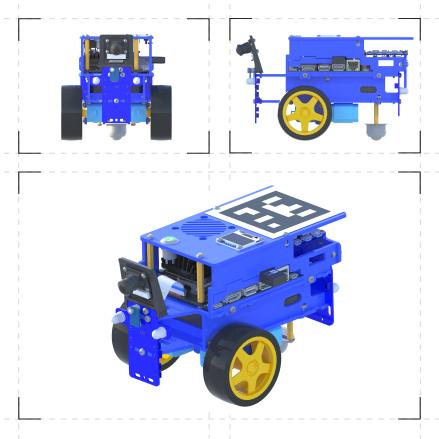
\includegraphics[width=0.5\textwidth]{d3.jpg}
    \caption{Robot Duckiebot.}
    \label{fig:robot-duckiebot}
\end{figure}

\subsection{Nadwozie}
Nadwozie robota Duckiebot jest w całości wykonane z plastikowych elementów. Taki wybór materiału na pewno obniża cenę robota ale ma też wpływ na jego wytrzymałość mechaniczną. Na rysunku \ref{fig:chassis-problem} przedstawiono typowe problemy nadwozia robotów Duckiebot.

\begin{figure}
    \centering
    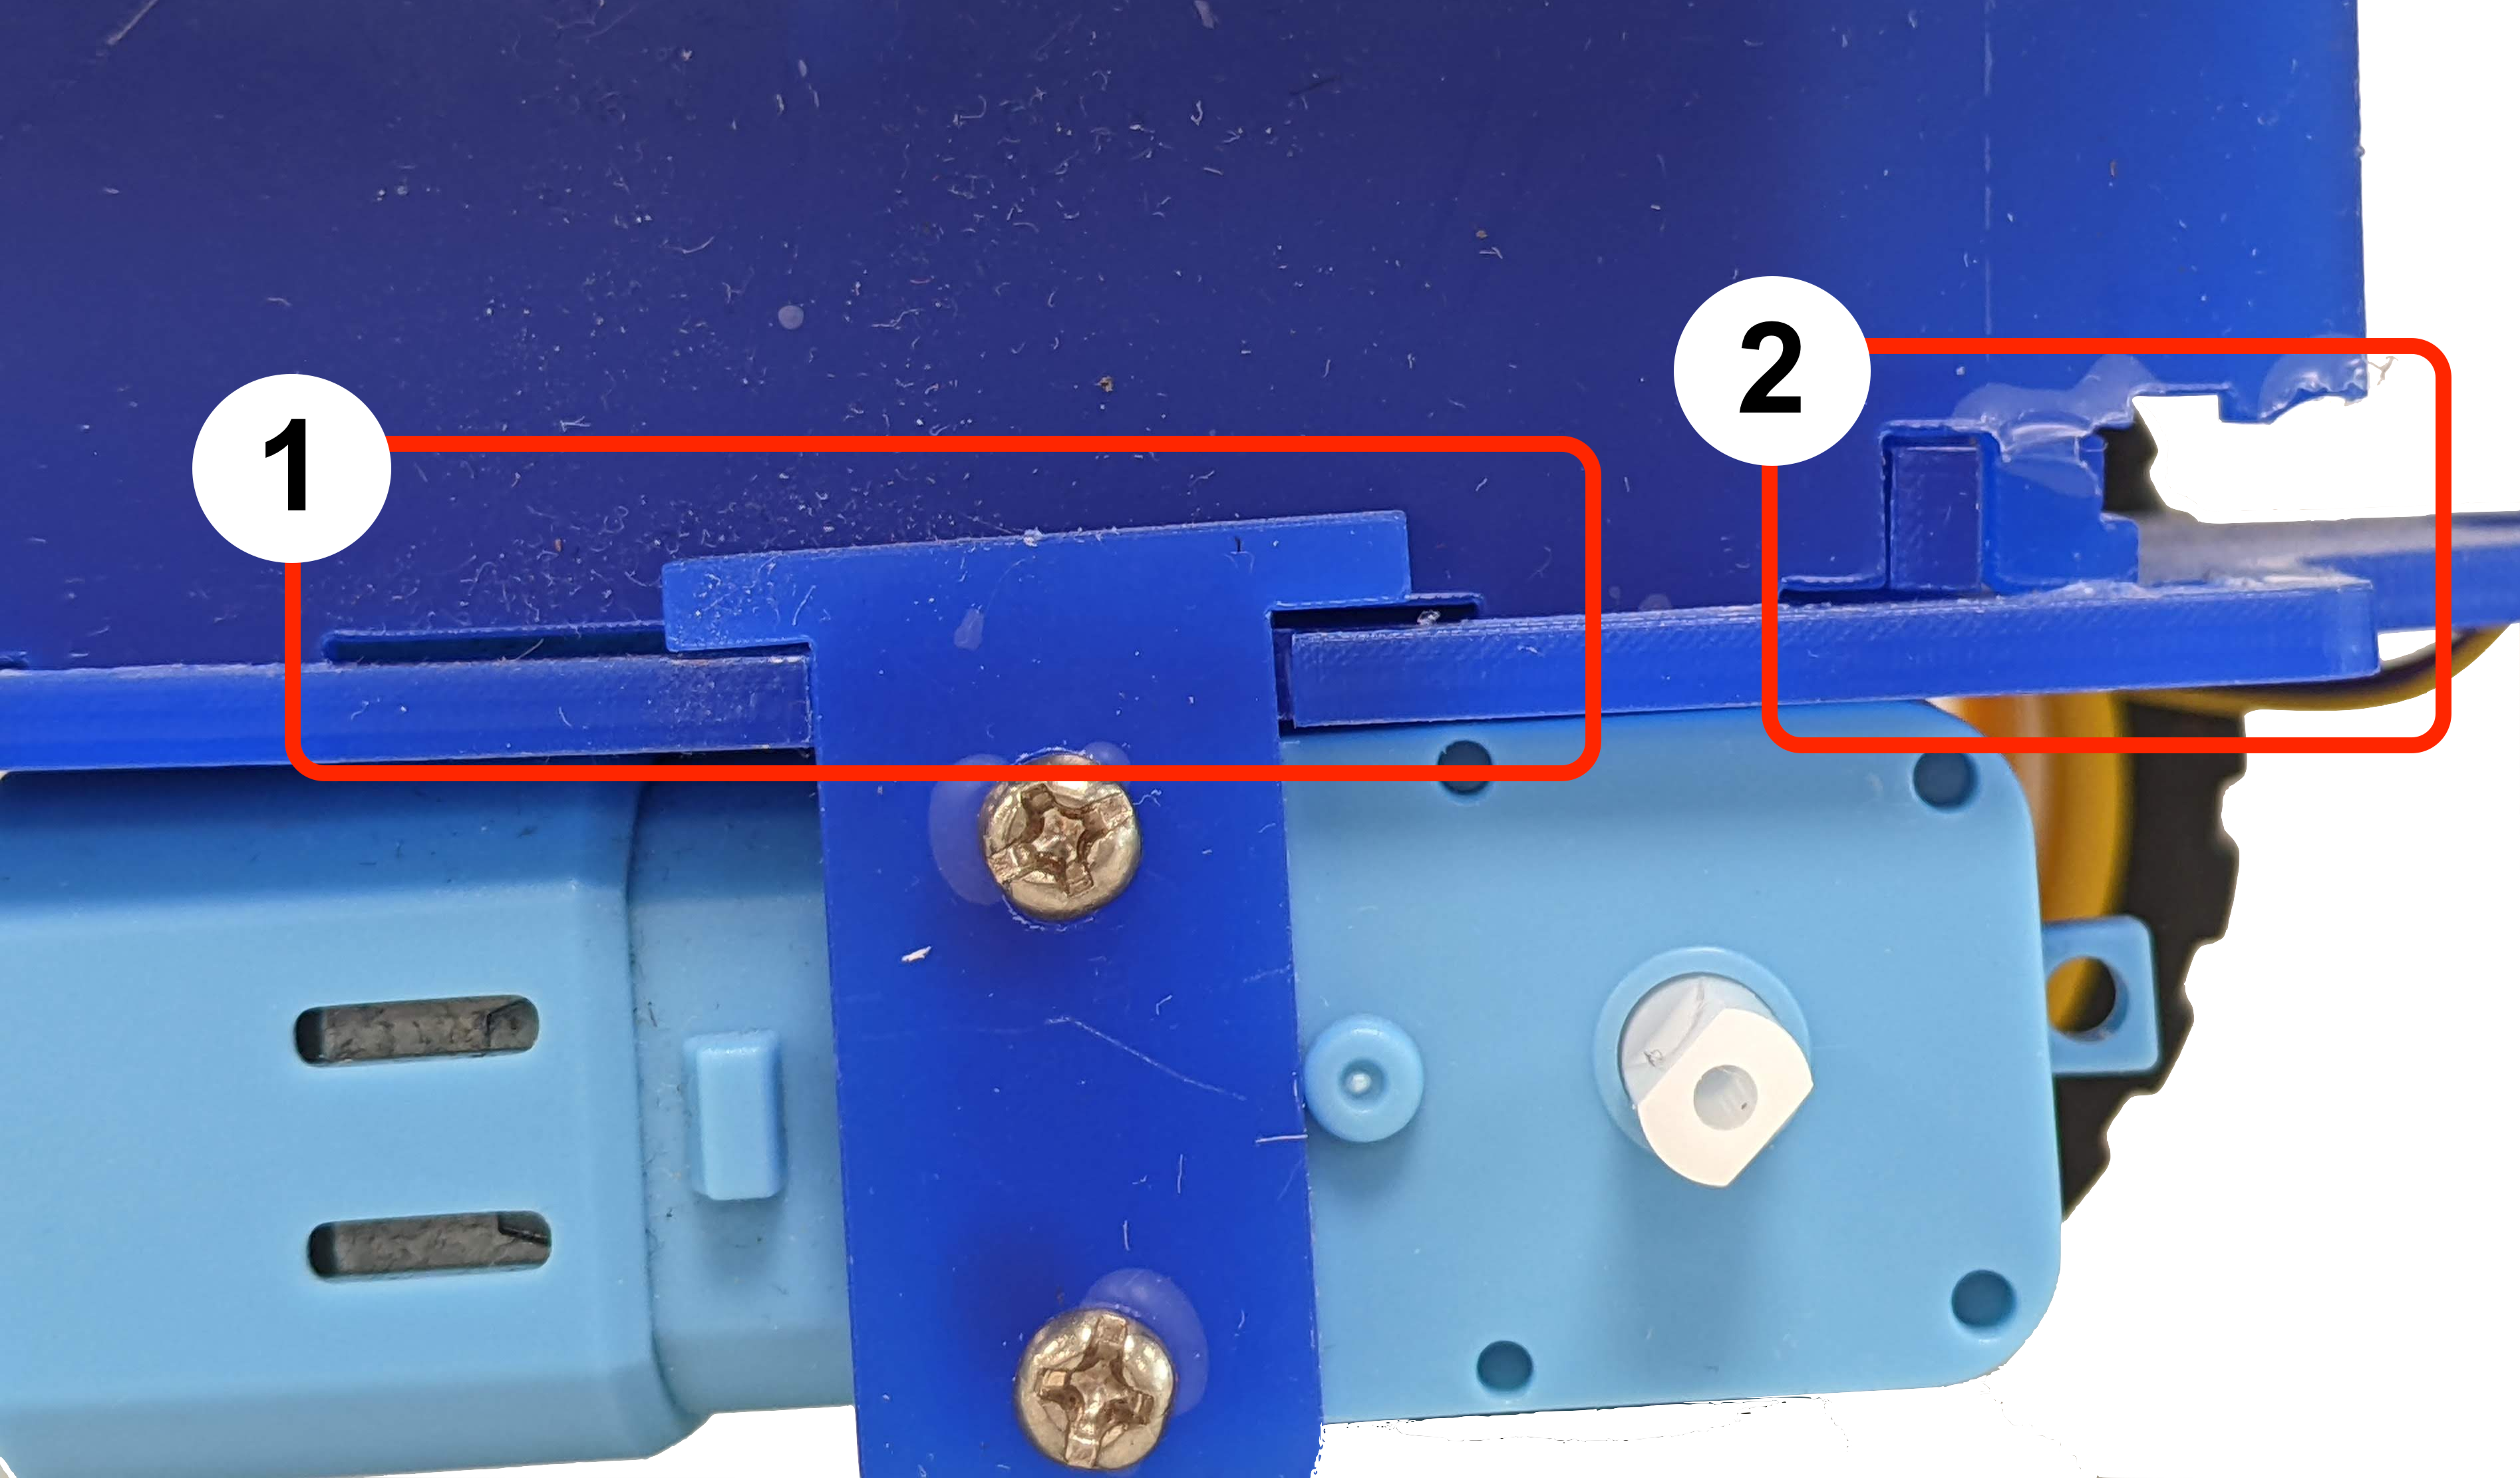
\includegraphics[width=0.7\textwidth]{chassis1.png}
    \caption{Fragment plastikowego nadwozia robota Duckiebot.}
    \label{fig:chassis-problem}
\end{figure}

Pierwszym z zauważonych problemów jest słaba jakość spasowania poszczególnych elementów nadwozia robota Duckiebot. Wynika ona, z niewystarczających rozmiarów przestrzeni w której znajduje się akumulator. W projekcie i wykonaniu nadwozia nie przewidziano, że nakrętki jakie znajdują się w tym miejscu także mają swoją wysokość przez co akumulator zajmuje trochę więcej miejsca niż to wynika z jego zewnętrznych wymiarów. Skutkuje to powstaniem szczelin (szczegół nr 1 na rys. \ref{fig:chassis-problem}) i mniej sztywnym mocowaniem silnika do nadwozia. Ze względu na właściwości mechaniczne materiału z jakiego wykonane jest nadwozie (plastik), oraz umiejscowienia otworów na nakrętki zbyt blisko krawędzi elementów nadwozia mają one tendencje do wyłamywania się (szczegół nr 2 na rys. \ref{fig:chassis-problem}). Pewnym mankamentem jest również zastosowanie śrub plastikowych (nie wszystkie) do połączeń elementów nadwozia.

Kolejnym problemem związanym z nadwoziem, jest brak odpowiedniej sztywności poprzecznej (wzdłuż osi Y) co skutkuje tym, 
że koła napędowe ulegają odkształceniu na zewnątrz (\emph{negative camber}), zob. rys. \ref{fig:negative-camber}. 

\begin{figure}
    \centering
    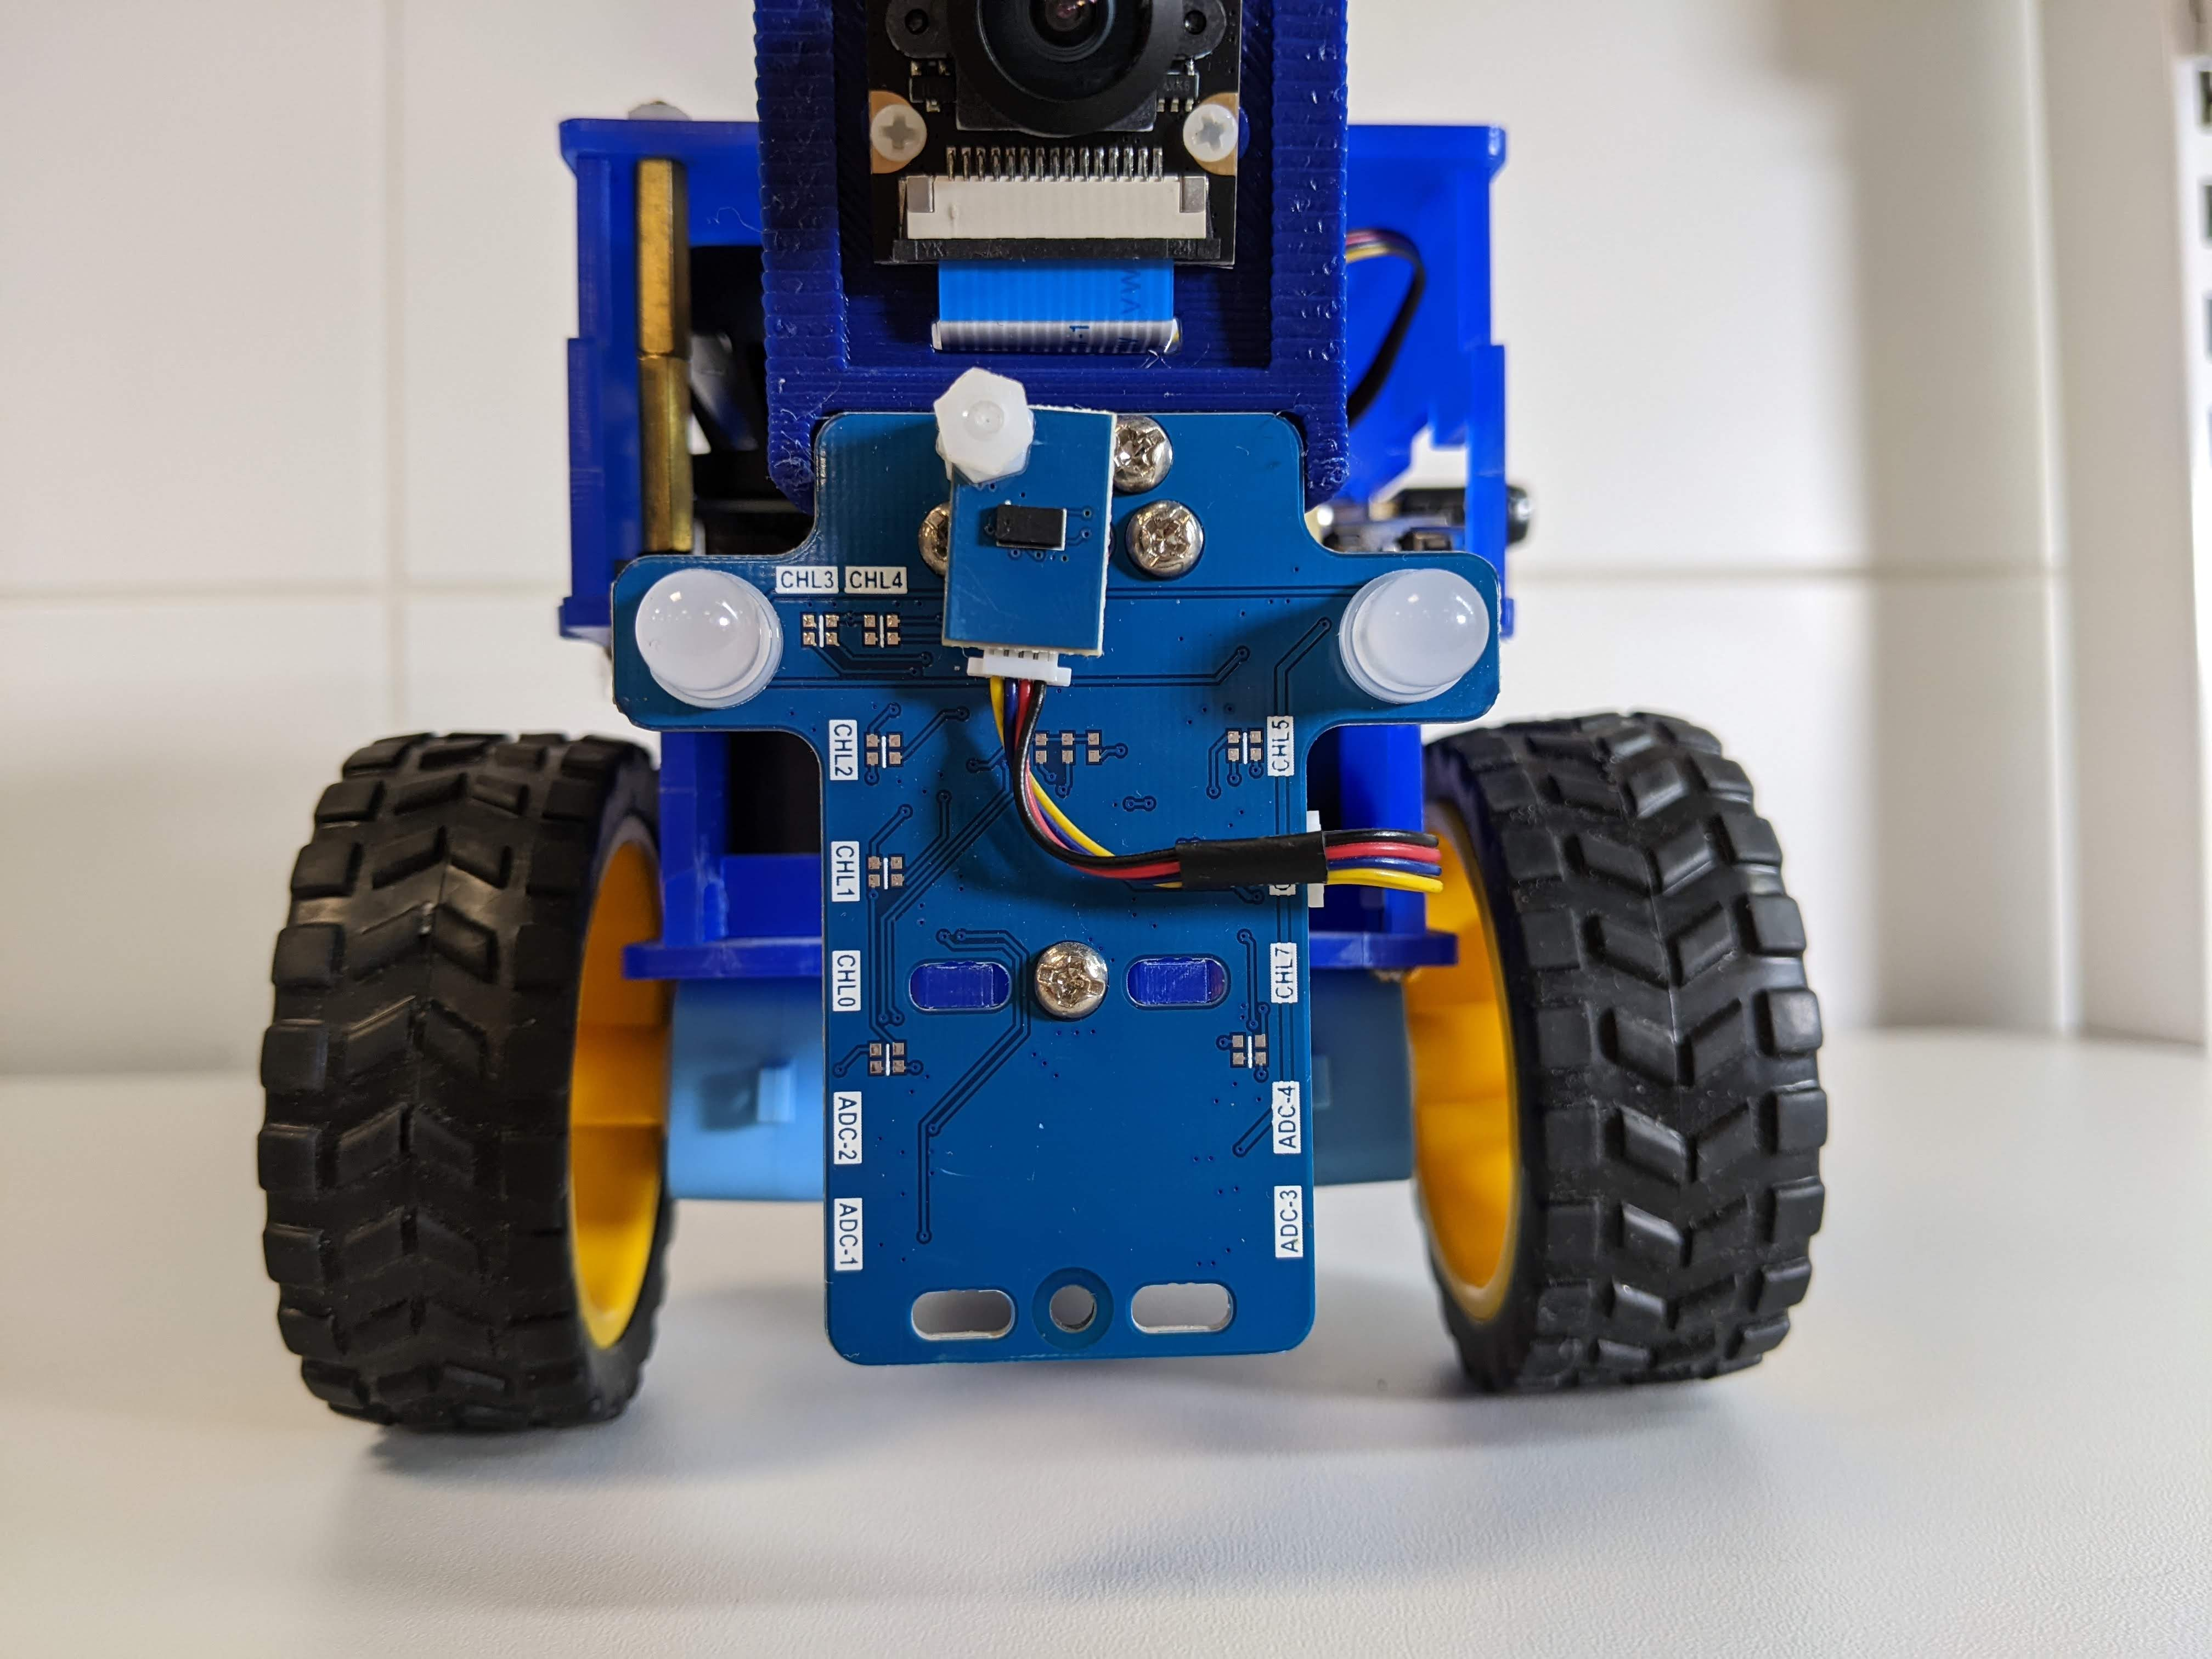
\includegraphics[width=0.7\textwidth]{PXL_20221207_092836283.png}
    \caption{Ujemny kąt pochylenia kół robota Duckiebot}
    \label{fig:negative-camber}
\end{figure}

Ujemny kąt pochylenia kół powoduje, że robot Duckiebot jest nadsterowny co na początku może się wydawać zaletą. Mając jednak na uwadze powierzchnię po jakiej porusza się robot Duckiebot (zobacz rodział \ref{subsec:plane}) oraz niesymetryczność w działaniu silników (przy tej samej wartości napięcia zasilania prędkości obrotowe silników nie są identyczne) zbyt duża sterowność jest wadą a nie zaletą. Powoduje ona iż nawet minimalne zakłócenie (pochodzące od nierównej nawierzchni i niesymetrycznej pracy silników) skutkują tym, że robot Duckiebot gwałtowanie zmienia kierunek ruchu tak, że układ sterowania nie jest w stanie poprawnie sterować robotem. 

Własności trakcyjne robotów Duckiebot można polepszyć łącząc mocowania silników poprzeczką która usztywnia mocowanie silników  zapobiegając ujemnym pochyleniom kół, zob. rys. \ref{fig:stiffening-crossbar}.

\begin{figure}[ht!]
    \centering
    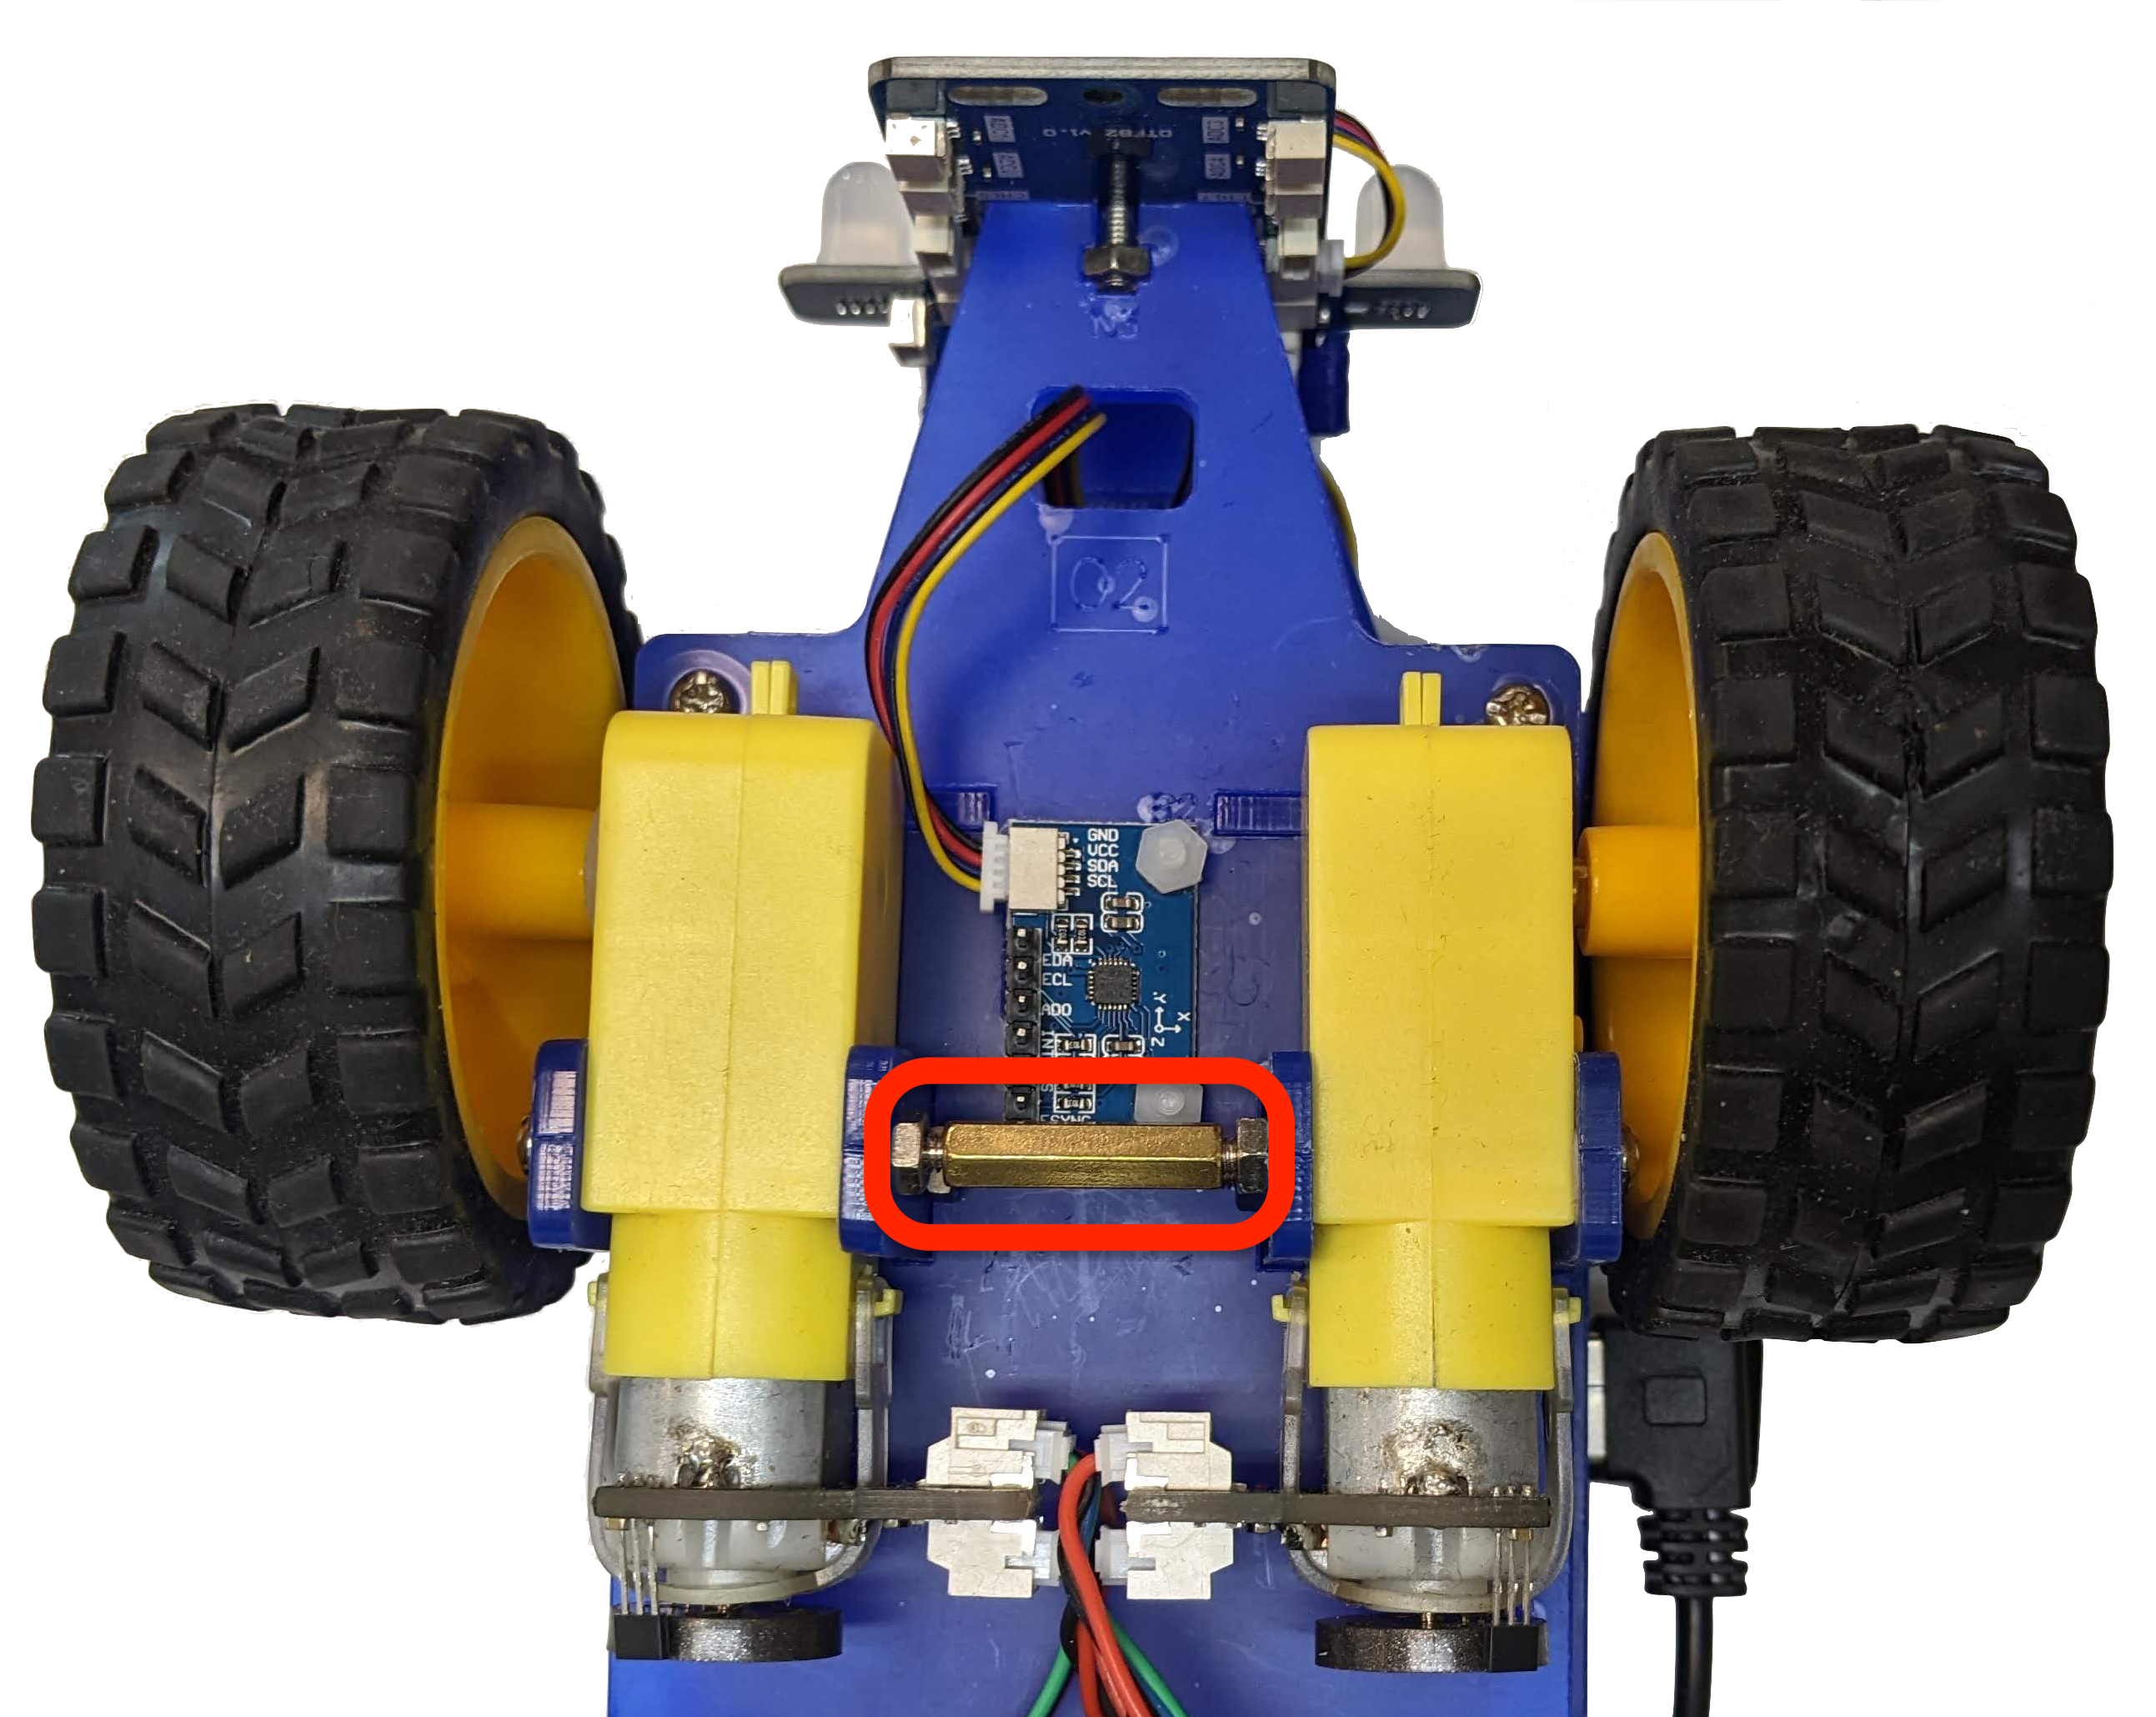
\includegraphics[width=0.7\textwidth]{drive-upgrade.png}
    \caption{Dodatkowa poprzeczka usztywniająca mocowanie silników robota Duckiebot.}
    \label{fig:stiffening-crossbar}
\end{figure}

Innym sposobem poprawienia właściwości trakcyjnych robotów Duckiebot jest wydrukowanie dodatkowego elementu\footnote{https://www.thingiverse.com/thing:2558770} który zapewnia współosiowość obydwu silników, zob. rys. \ref{fig:stiffening-element}

\begin{figure}[ht!]
    \centering
    \includegraphics[width=0.7\textwidth]{img/duckie\_th.jpeg}
    \caption{Dodatkowy element usztywniająca mocowanie silników robota Duckiebot.}
    \label{fig:stiffening-element}
\end{figure}

Zredukowanie ujemnego kąta pochylenia kół skutkuje, znaczną poprawą właściwości trakcyjnych robota Duckiebot. Nie jest on tak wrażliwy na zakłócenia i nie zmienia kierunku jazdy w sposób gwałtowny. Na rysunku \ref{fig:wheel-contact} przedstawiono efekt wykorzystania dodatkowej poprzeczki łączącej silniki robota. Można zauważyć, że po zastosowaniu poprzeczki koła robota Duckiebot przylegają do powierzchni całą swoją szerokością zapewniając lepsze właściwości trakcyjne.

\begin{figure}[ht!]
    \centering
    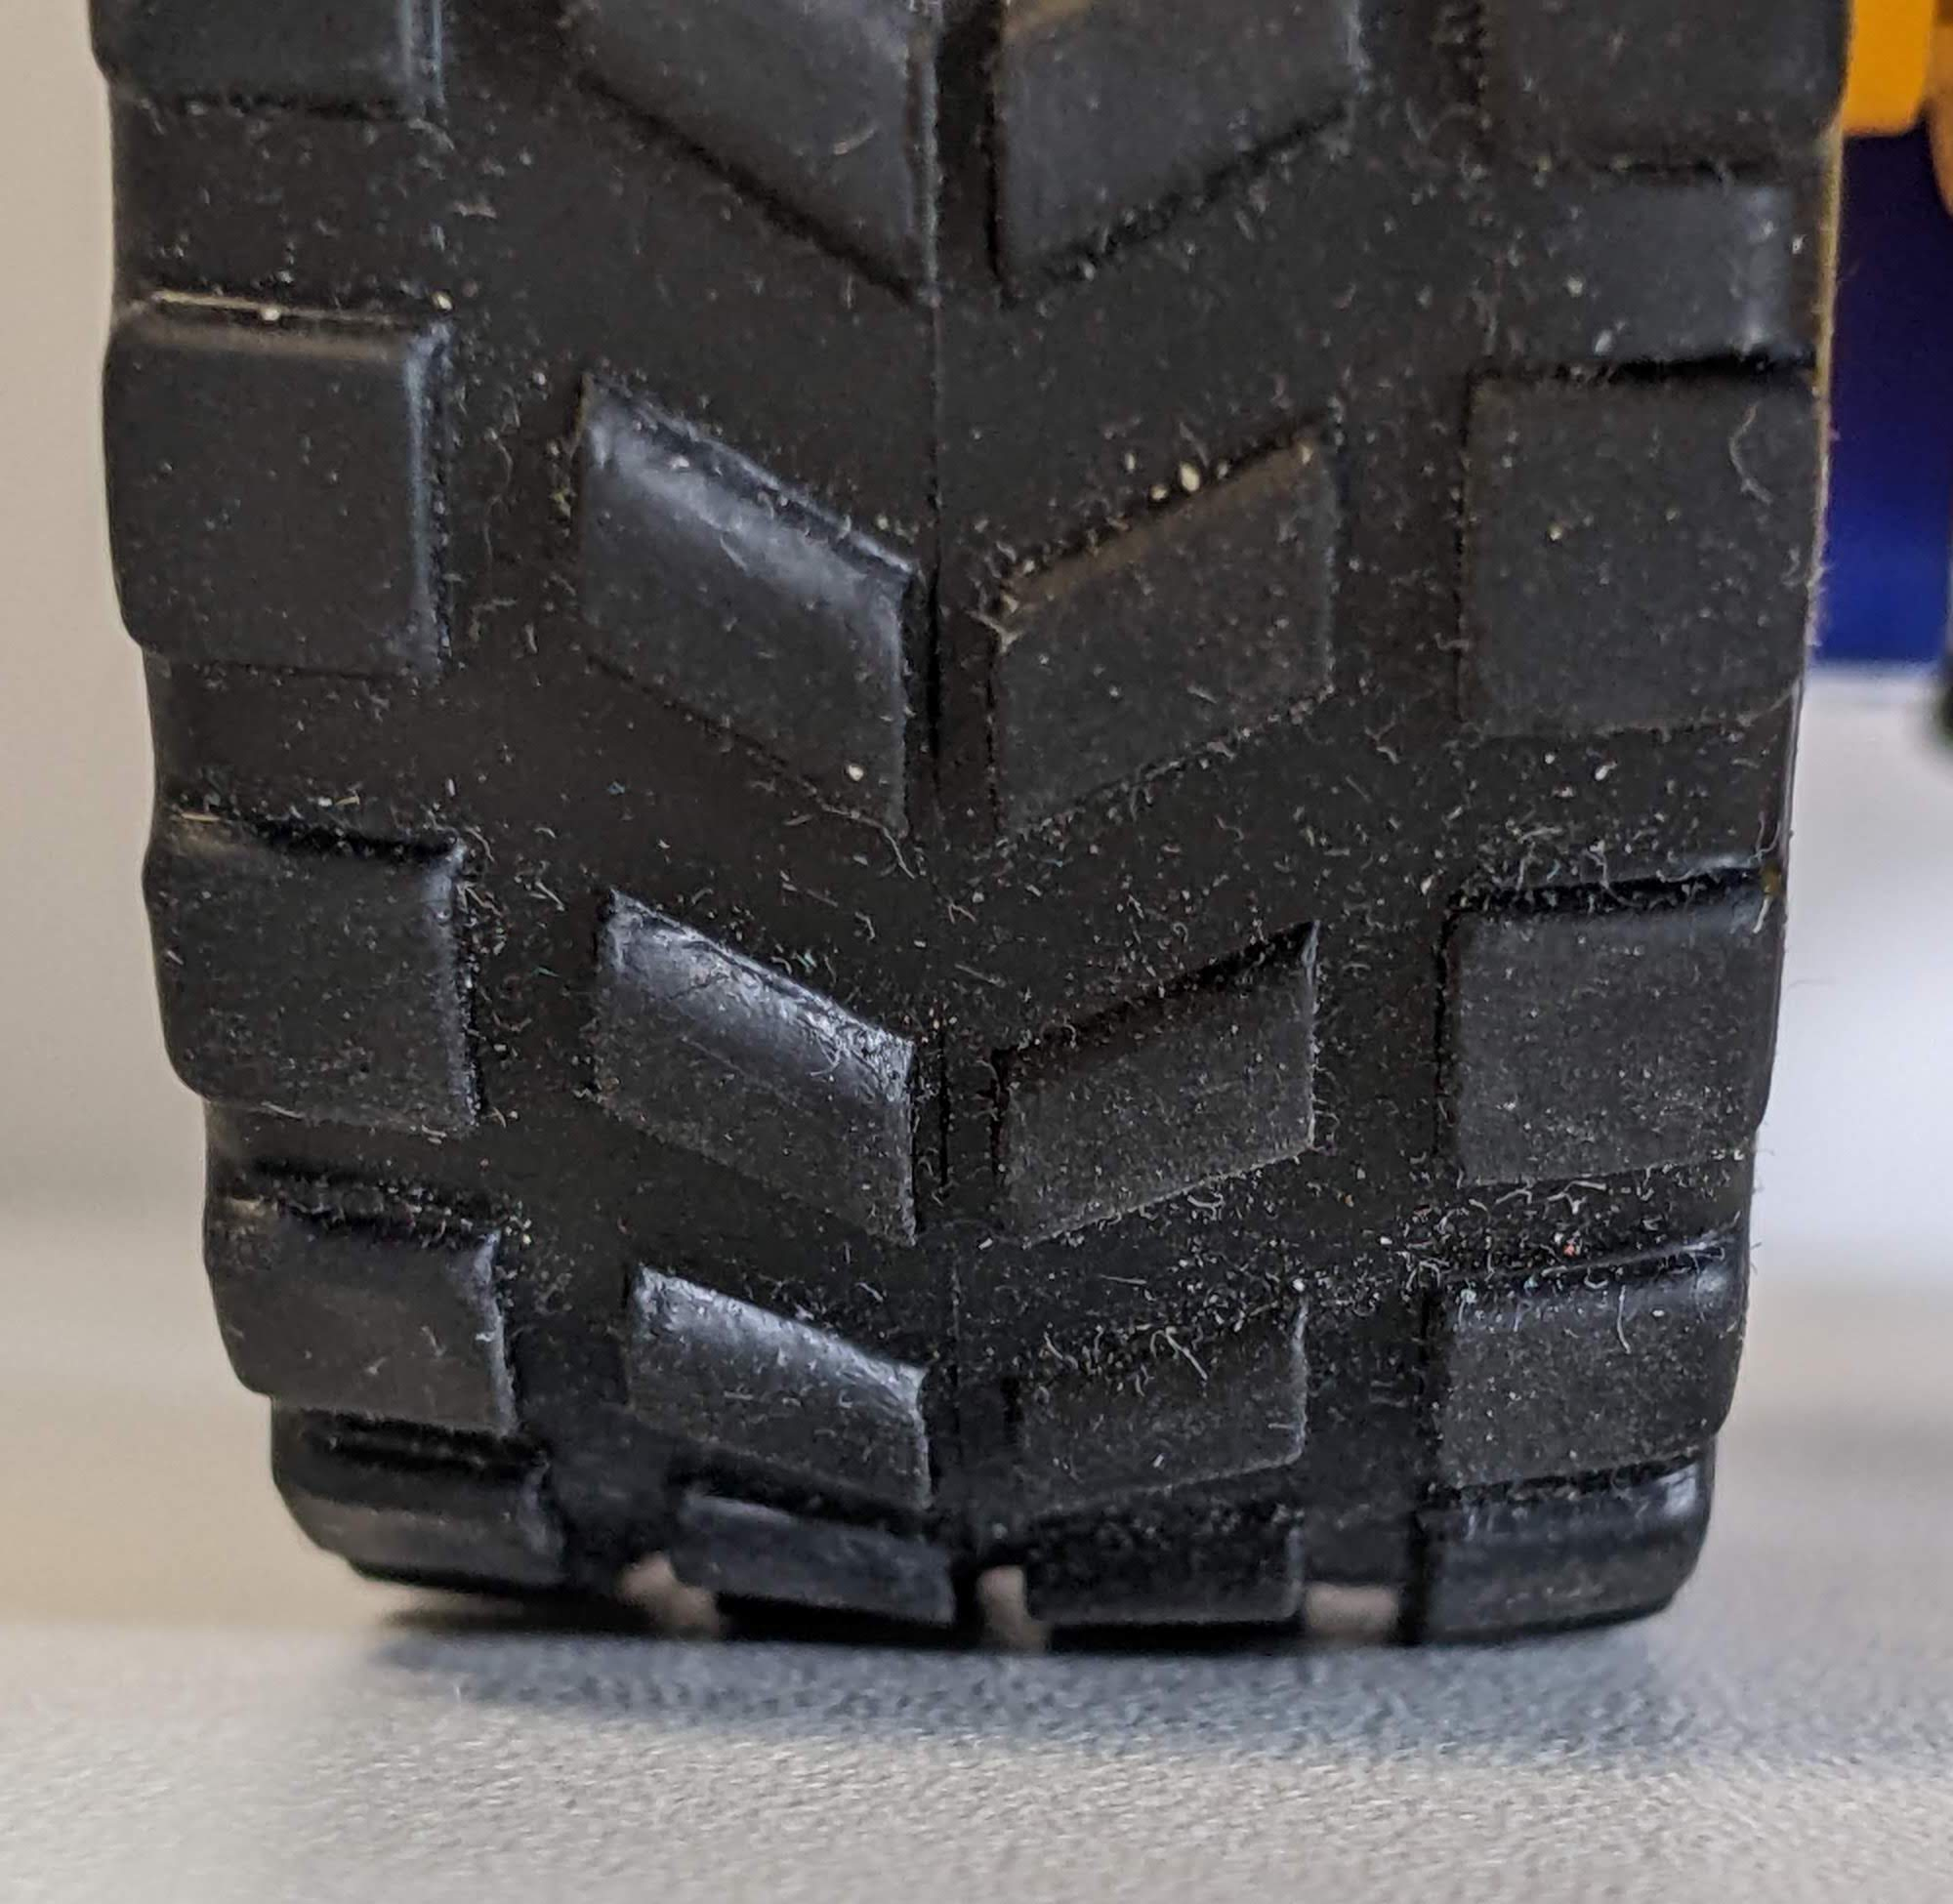
\includegraphics[width=0.45\textwidth]{wheel-contact-1.jpg}
    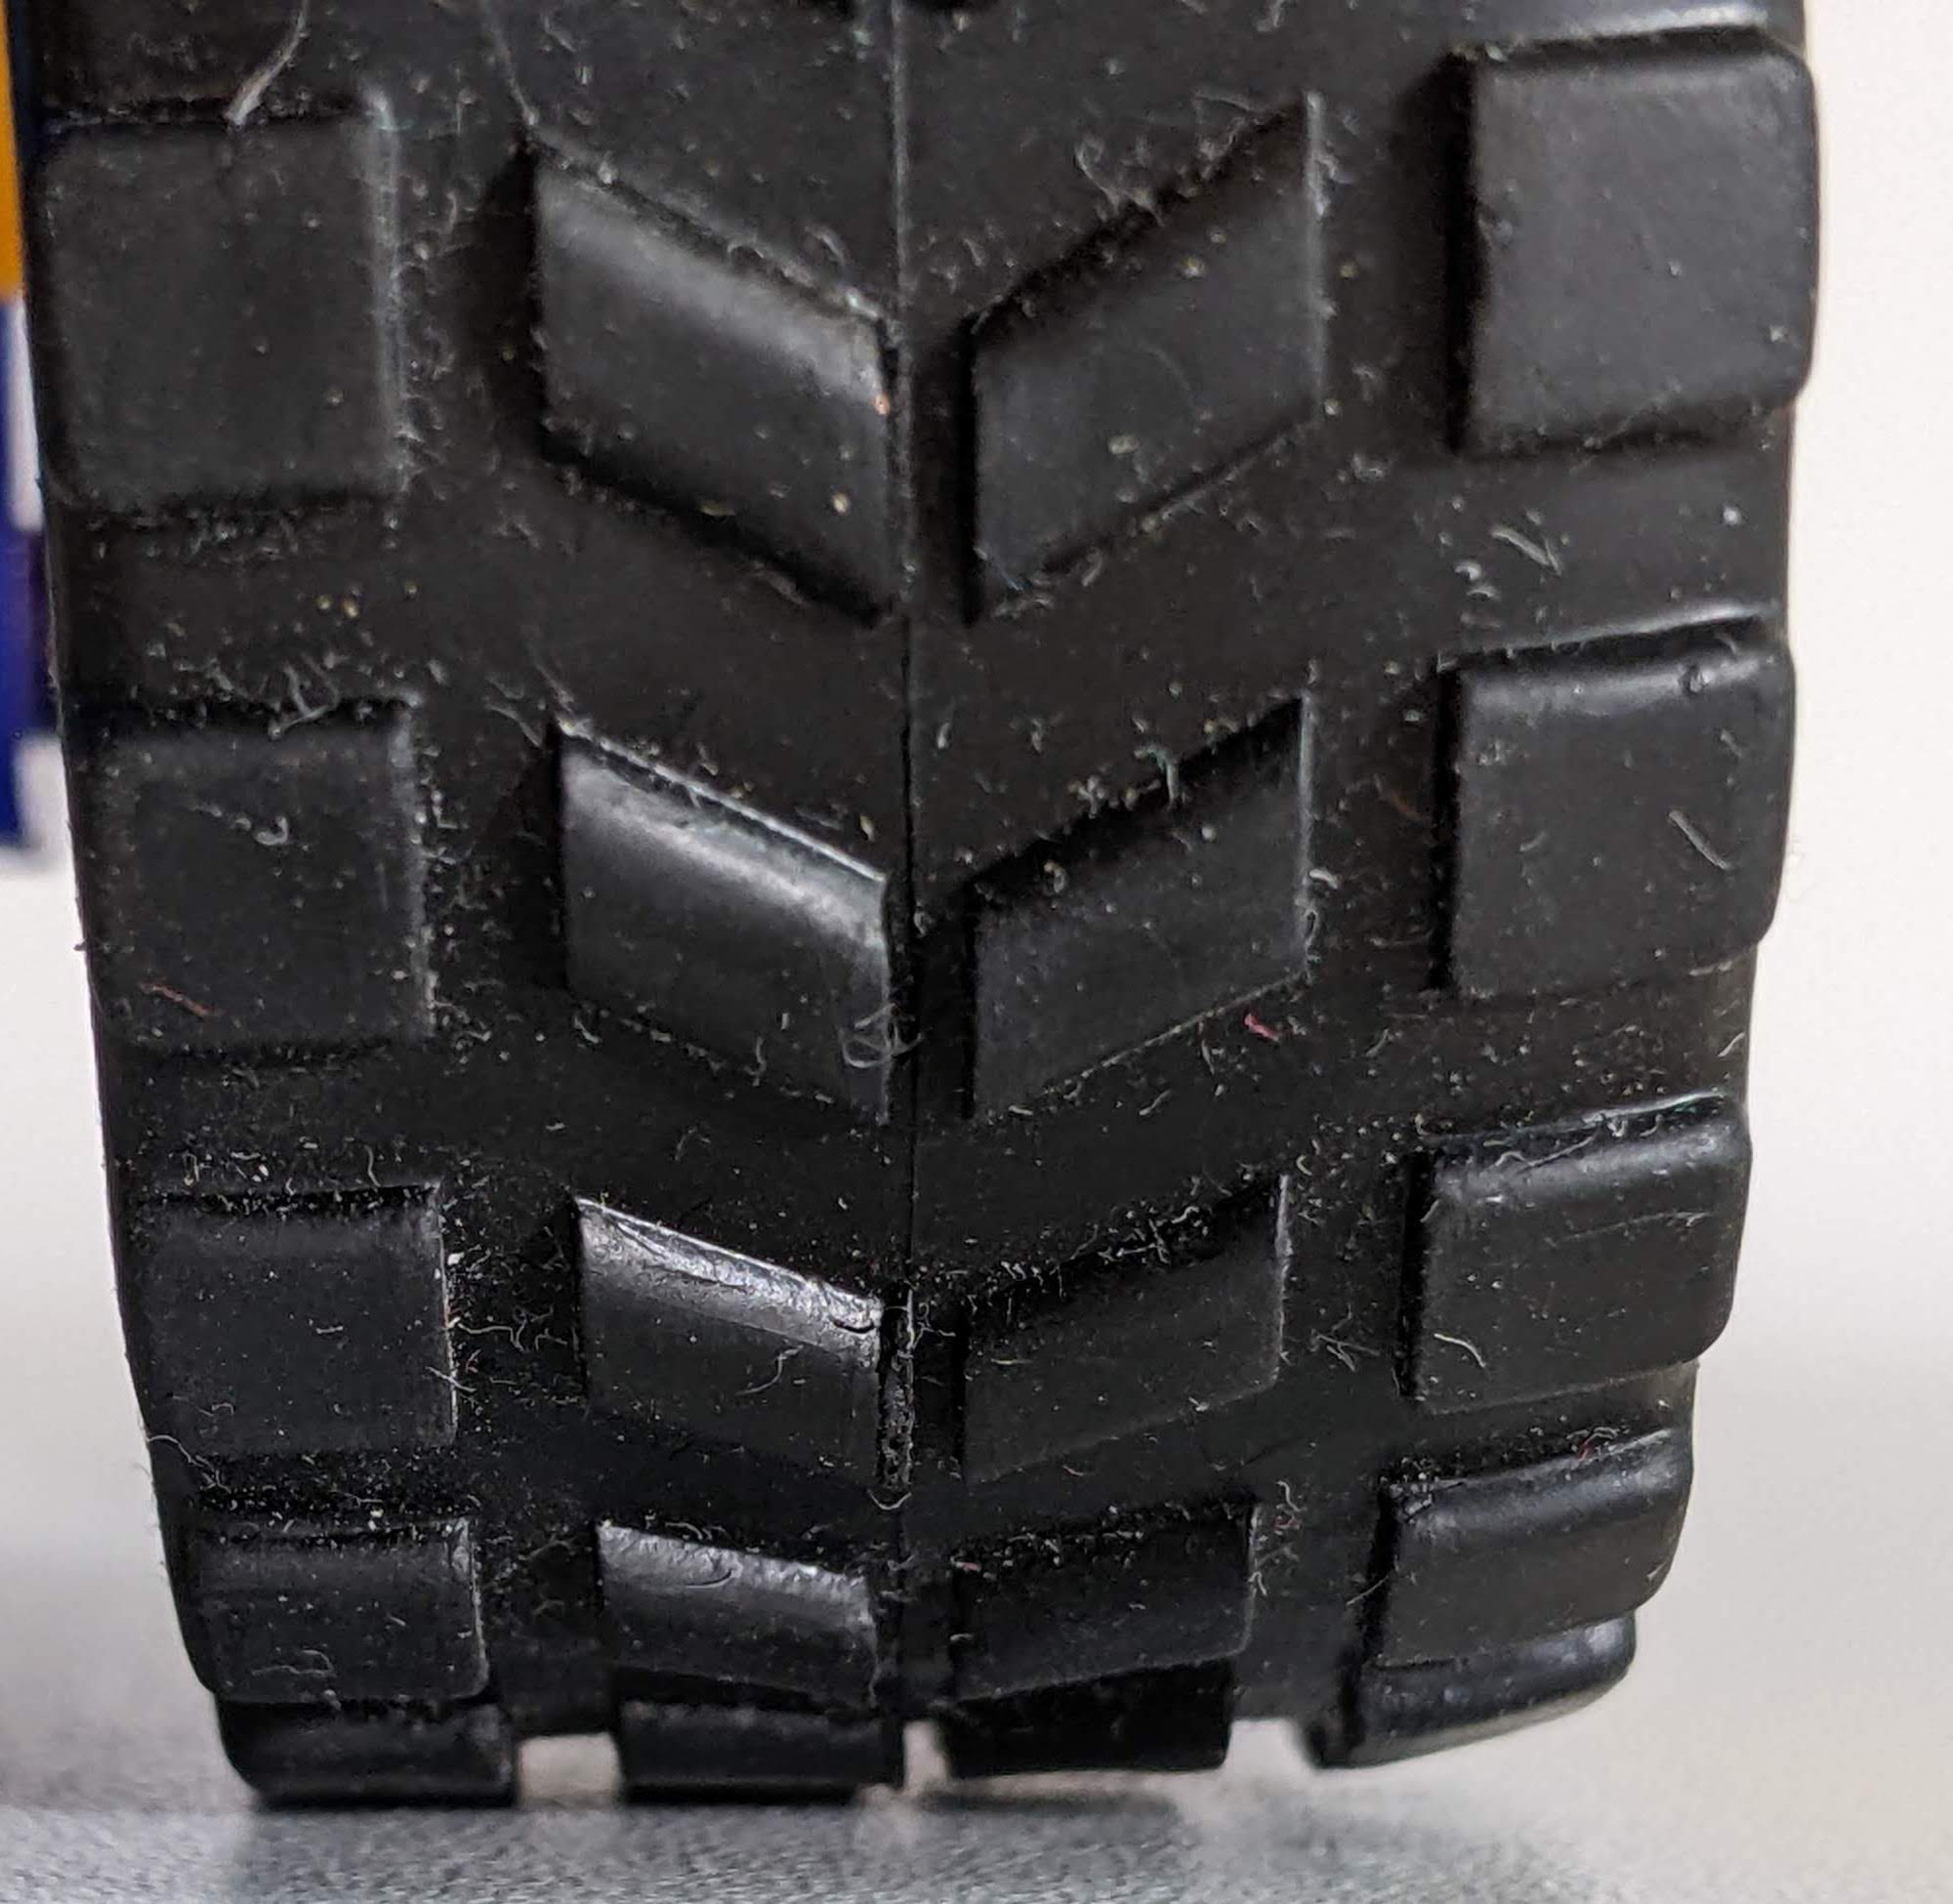
\includegraphics[width=0.45\textwidth]{wheel-contact-2.jpg}
    \caption{Rezultat wykorzystania poprzeczki usztywniającej mocowanie silników na koła robota Duckiebot.}
    \label{fig:wheel-contact}
\end{figure}

\subsection{Silniki}
W oryginalnie w robotach Duckiebot używa się silników DG01D-E z przekładnią 48:1, 90 obr/min i momencie obrotowym 0.078 Nm przed przekładnią i momencie 3.744 Nm po przekładni.
Sinik DG01D-E wyposażony jest również w enkoder kwadraturowy o prawdopodobnej rozdzielczości 8 impulsów na obrót (producent nie udostępnia takiej informacji) przed przekładnią i 576 impulsów po przekładni. Silnik DG01D-E charakteryzuje się dużą prędkością obrotową ale niezbyt dużym momentem, zob. tabela \ref{table:dc-motors-summaery}. Uwzględniając niedoskonałości makiety, zob. rozdział \ref{subsec:plane}, a w szczególności różne wysokości pomiędzy poszczególnymi panelami (zob. rys. \ref{fig:smart-city-plan-1}) powodowało to, że robot Duckiebot potrafił się zatrzymać podczas przejazdu z jednego panelu na drugi.

% https://ros-mobile-robots.com/DG01D-E-motor-with-encoder/
% https://www.cuidevices.com/blog/what-is-encoder-ppr-cpr-and-lpr
Silniki w robotach Duckiebot zostały zastąpione silnikami SJ01 (SKU:FIT0450) z przekładnią 120:1, 160 obr/min i momencie obrotowym 0.07Nm przed przekładnią i momencie 8.4 Nm po przekładni. Dodatkowo silnik SJ01 jest wyposażony w enkoder kwadraturowy o rozdzielczości 8 impulsów na obrót przed przekładnią i 960 impulsów na obrót po przekładni.  

Obydwa silniki mają takie same wymiary zewnętrzne, obudowy oraz otwory montażowe więc ich wymiana nie stanowi problemu. Należy jedynie zwrócić uwagą na prawidłowe podłączenie sygnałów sterowania silnikiem i sygnałów od enkoderów ponieważ w silniku DG01D-E wszystkie sygnały zintegrowane są w jednym 6-cio pinowym złączu, natomiast w silniku SJ01 są złącza: jedno do zasilana a drugie to enkodera.

W tabeli \ref{table:dc-motors-summaery} zamieszczono wszystkie parametry silników DG01D-E oraz SJ01. 

\def\arraystretch{1.5}
\setlength{\tabcolsep}{0.01\textwidth}
\begin{table}[ht!]
\begin{center}
    \begin{tabular}{|c|c|c|c|c|c|c|c|}
    \hline
         \multirow{3}{*}{\thead{Typ silnika}} & \multirow{3}{*}{n} & \multicolumn{3}{|c|}{przed przekładnią} & \multicolumn{3}{|c|}{po przekładni} \\ \cline{3-8}
         
         & & $\omega$ & moment & enkoder  & $\omega$ & moment & enkoder  \\
         
         & & [obr/min] & [Nm] & [imp/obr]  & [obr/min] & [Nm] & [imp/obr]  \\
         \hline \hline
         DG01D-E & 48:1 & 90  & 0.078  & 12   & 1.874 & 3.744  & 576  \\ 
         \hline
         SJ01 & 90:1 & 120  & 0.070  & 8 & 1.333  & 8.400  & 960 \\ 
         \hline
    \end{tabular}
    \caption{\label{table:dc-motors-summaery}Podsumowanie parametrów silników robota Duckiebot.}
\end{center}
\end{table}

Ostatecznie silnik SJ01, pomimo nieznacznie mniejszego momentu obrotowego przed przekładną, jest zdecydowanie lepszym wyborem niż silnik DG01D-E. Finalnie posiada większy moment obrotowy oraz enkoder o większej rozdzielczości co zdecydowanie polepsza właściwości jezdne robota Duckiebot oraz dokładność sterowania prędkością obrotową silnikami. Nieznacznie mniejsza prędkość obrotowa $\omega$ po przekładni nie ma żadnego znaczenia, ponieważ roboty Duckiebot nie są robotami które mają brać udział w wyścigach robotów ale mają w sposób inteligenty poruszać się po makiecie miasta.

\todo{Sprawdzić czy SJ01 ma metalowy wał, jeśli tak dodać zanie, że można dodatkowo przykręcić koła do }

%\href{https://botland.com.pl/silniki-dc-z-przekladnia-i-enkoderami/6287-silnik-z-przekladnia-sj01-120-1-6v-160rpm-enkoder-5904422306793.html}{Botland}, \href{https://www.dfrobot.com/product-1457.html}{DFRobot}

\subsection{Bateria}
W robotach Duckiebot zastosowano akumulator litowo jonowy o pojemności 10Ah. Obudowa akumulatora zawiera również zabudowany układ elektroniczny który steruje pracą baterii np. nie dopuszcza do nadmiernego jej rozładowania co jak wiadomo jest szkodliwe dla tego typu akumulatorów. Samo sterowanie pracą baterii jest dużo bardziej złożone o czym można się przekonać analizując maszynę stanów realizowaną przez układ elektroniczny baterii, zob. rys. \ref{fig:battery-state-machine}.

\begin{figure}[ht!]
    \centering
    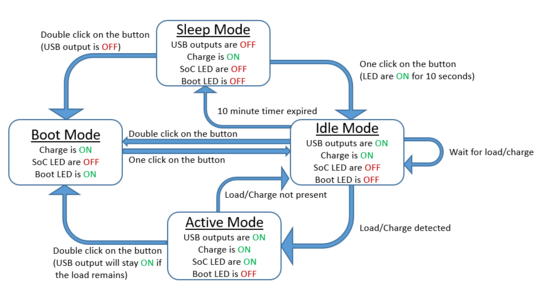
\includegraphics[width=0.85\textwidth]{BatteryStateMachine.png}
    \caption{Maszyna stanów zaimplementowana w układzie elektronicznym akumulatora robota Duckiebot.}
    \label{fig:battery-state-machine}
\end{figure}

Stan naładowania baterii oraz aktualny stan maszyny stanów w jakim się znajduje bateria jest prezentowany za pomocą 4 diod led zamontowanych na obudowie. Jest to rozwiązanie prost ale i skuteczne. Niestety w samym robocie Duckiebot bateria zabudowana jest w taki sposób, że diody sygnalizujące stan baterii są nie widoczne, przez co w żaden sposób nie można określić np. stopnia rozładowania baterii robota Duckiebot. Jest również możliwość programowego odczytania poziomu naładowania baterii robota Duckiebot, niestety bardzo często ta funkcjonalność nie działa prawidłowo. Najprostszym rozwiązaniem tego problemu jest zmiana sposoby zabudowania akumulatora w robocie Duckiebot tak aby jego stan można było zawsze odczytać korzystając z diód zamontowanych na obudowie. 

%\subsection{Koła}
%Koła mają tą wadę, że po pewnym czasie mogą odpaść od wału silnika. Brak jakiejkolwiek możliwości mechanicznego zabezpieczenia przed taką sytuacją. Problem można rozwiązać przy zastosowaniu silników SJ01 na dwa sposoby
%\paragraph{Rozwiązanie 1}
%Zakup innych typów kół np. \href{https://www.dfrobot.com/product-652.html}{SKU:FIT0199-B} (wymagany dodatkowo  adaptera który nie jest już produkowany \href{https://www.dfrobot.com/product-645.html}{SKU:FIT0198}) lub \href{https://www.dfrobot.com/product-1535.html}{SKU:FIT0500} (większa średnica kół). Można również zakupić koła z firmy Botland \href{https://botland.com.pl/kola-z-oponami/12463-kolo-65x15-mm-biale-5903351248143.html}{DNG-12463}, \href{https://botland.com.pl/kola-z-oponami/13946-kolo-z-opona-65x13mm-biale-5903351248174.html}{DNG-13946}.

%\paragraph{Rozwiązanie 2}
%Wywiercenie otworów w standardowych kołach (SKU:FIT0003) i przykręcenie ich śruba do wału silnika

\subsection{Makieta}\label{subsec:plane}
Głównym składnikiem/elementem projektu Duckietown jest makieta. W założeniu ma ona modelować kształt drogi, układ skrzyżowań po której poruszają się roboty Duckiebot. Linie proste i łuki oznakowane liniami w kolorze białym i żółtym natomiast skrzyżowania oznakowane są czerwonymi liniami. Trasa po której poruszają się roboty Duckiebot może być dowolnie konfigurowana przez odpowiednie ułożenie elementów makiety. Podstawowym elementem z której zbudowana jest trasa jest gumowo-piankowy mata. Pierwszym z problemów są odklejające się elementy taśmy wykorzystywane o oznaczania linii, zob. rys. \ref{fig:smart-city-plan-1}. Drugim problem jest sama jakość wykonania mat gumowo-piankowych, . Maty z jednego opakowania mają różną wysokość co skutkuje tym, że poruszające się po nich roboty Duckiebot zmieniają w sposób zupełnie przypadkowy kierunek swojej jazdy, zob. rys. \ref{fig:smart-city-plan-1}.

\begin{figure}[ht!]
    \centering
    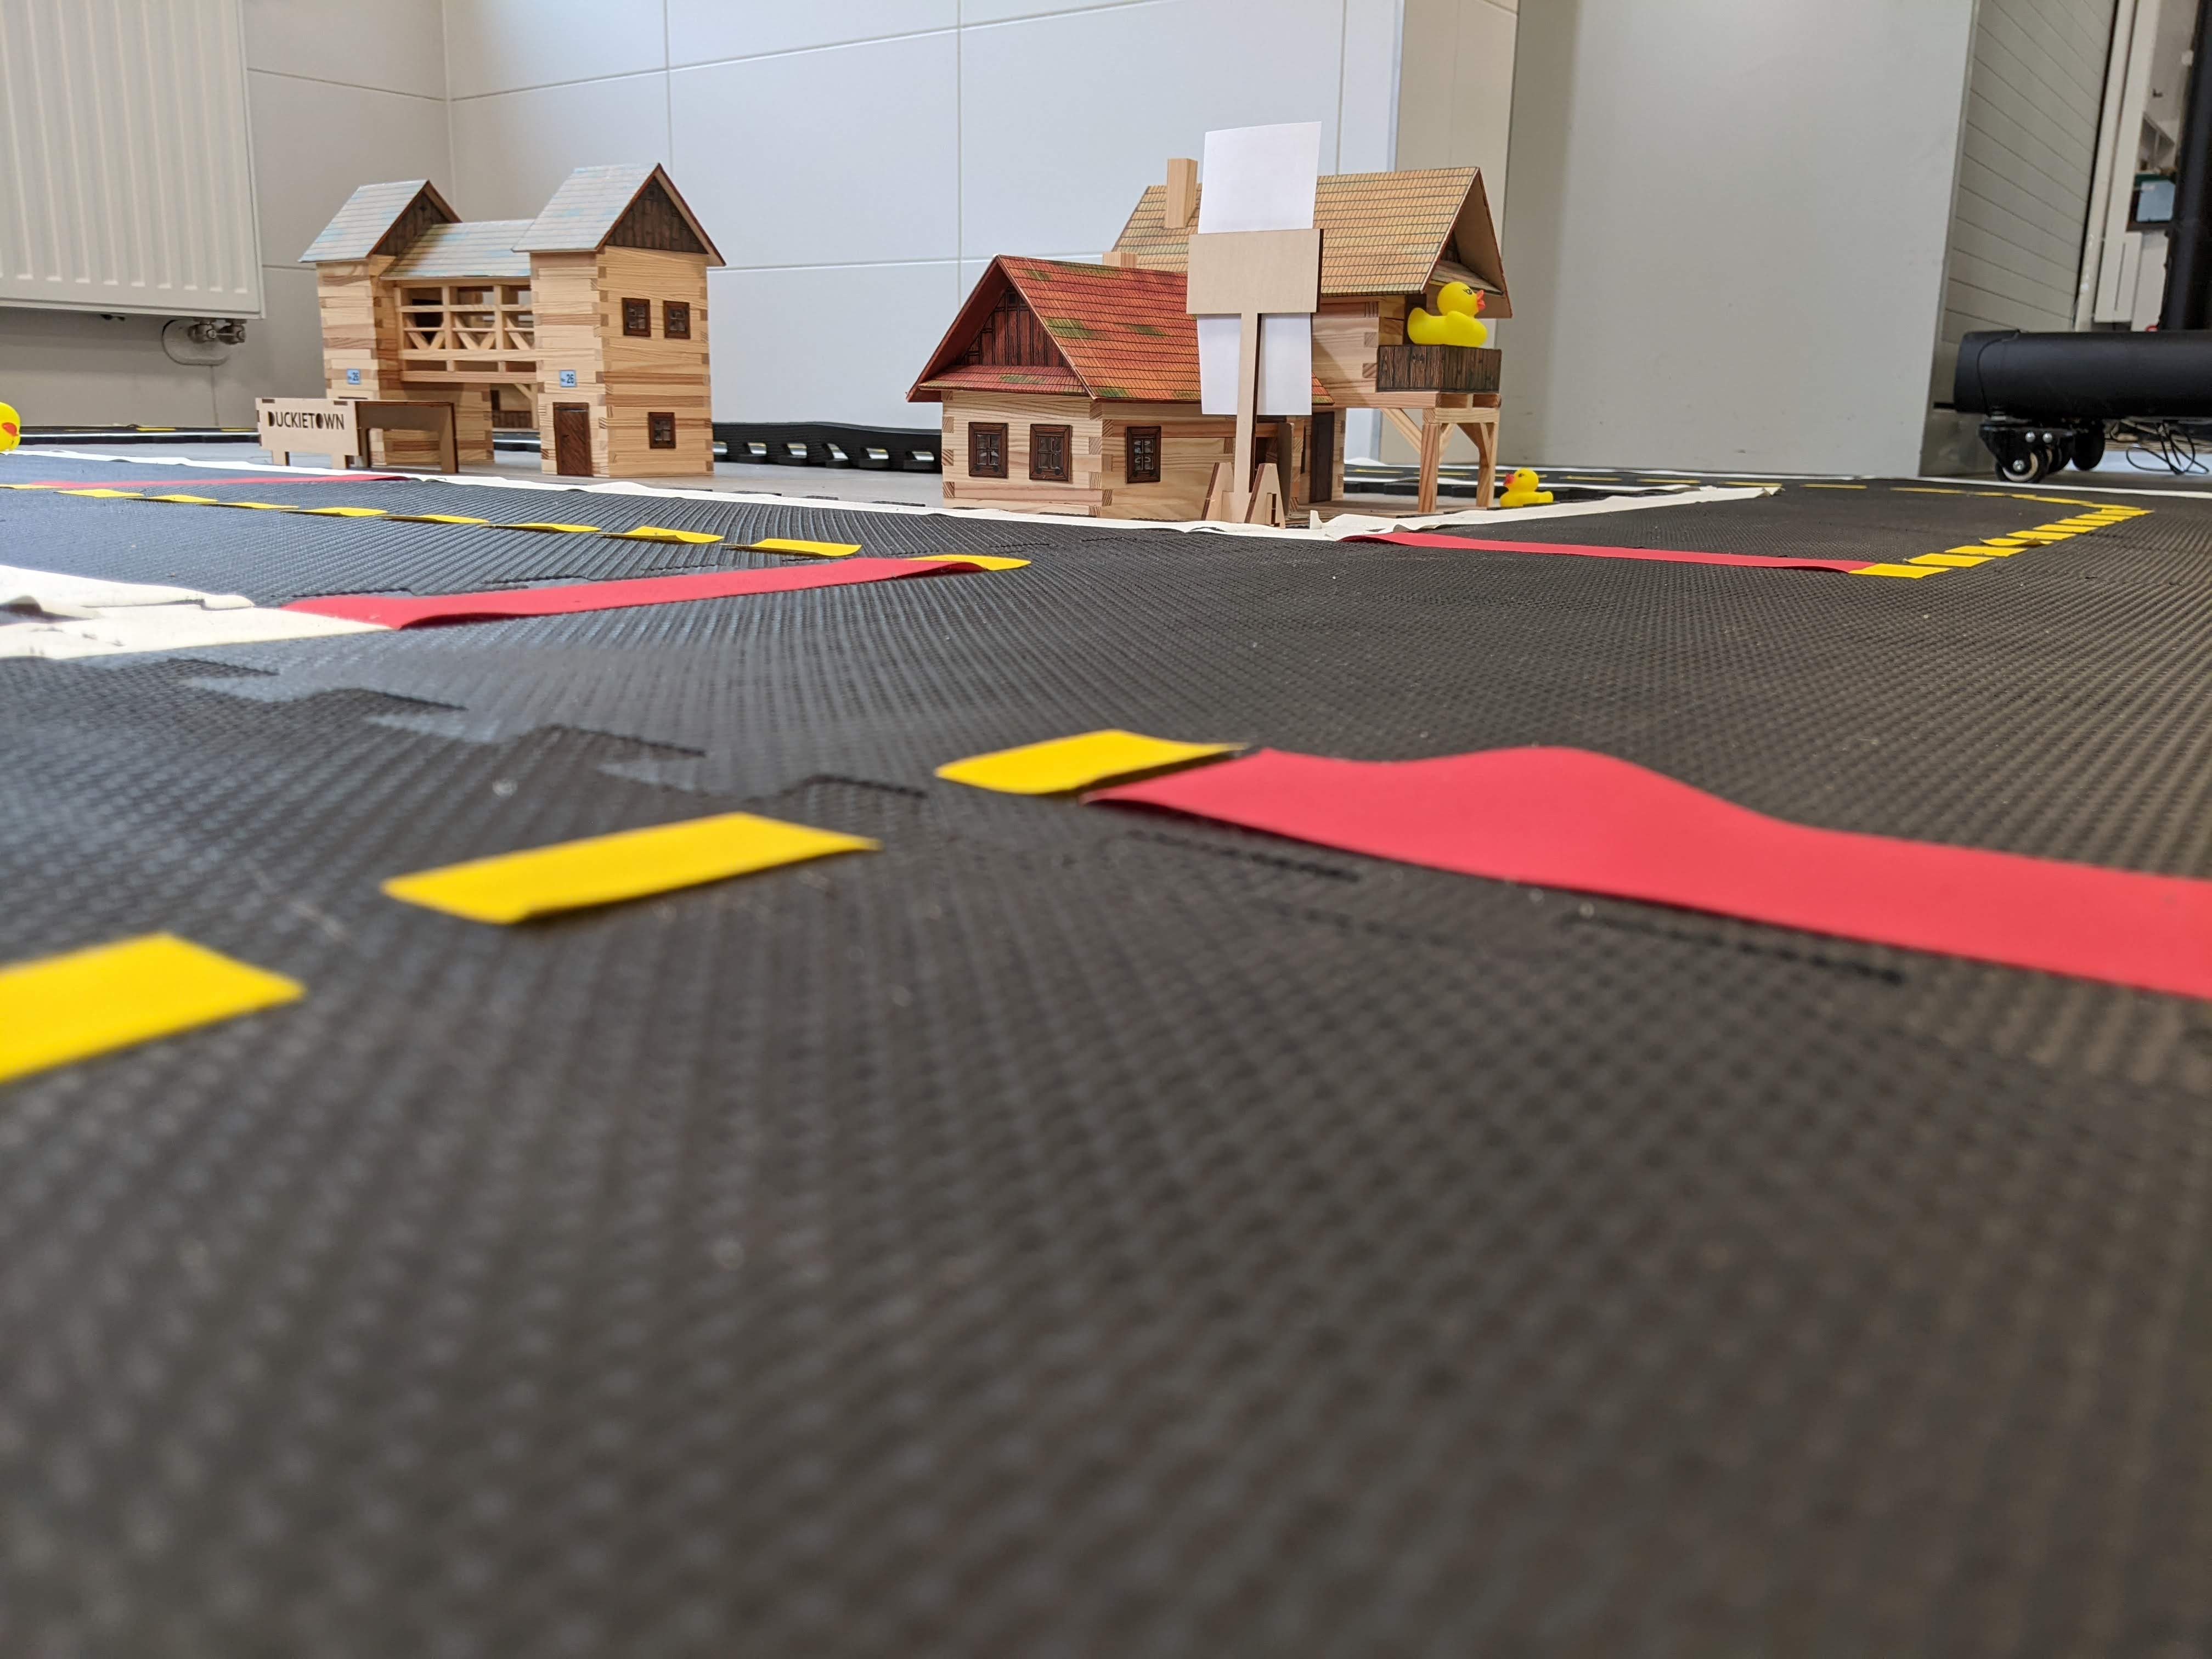
\includegraphics[width=0.4\textwidth]{floor-1.jpg}
    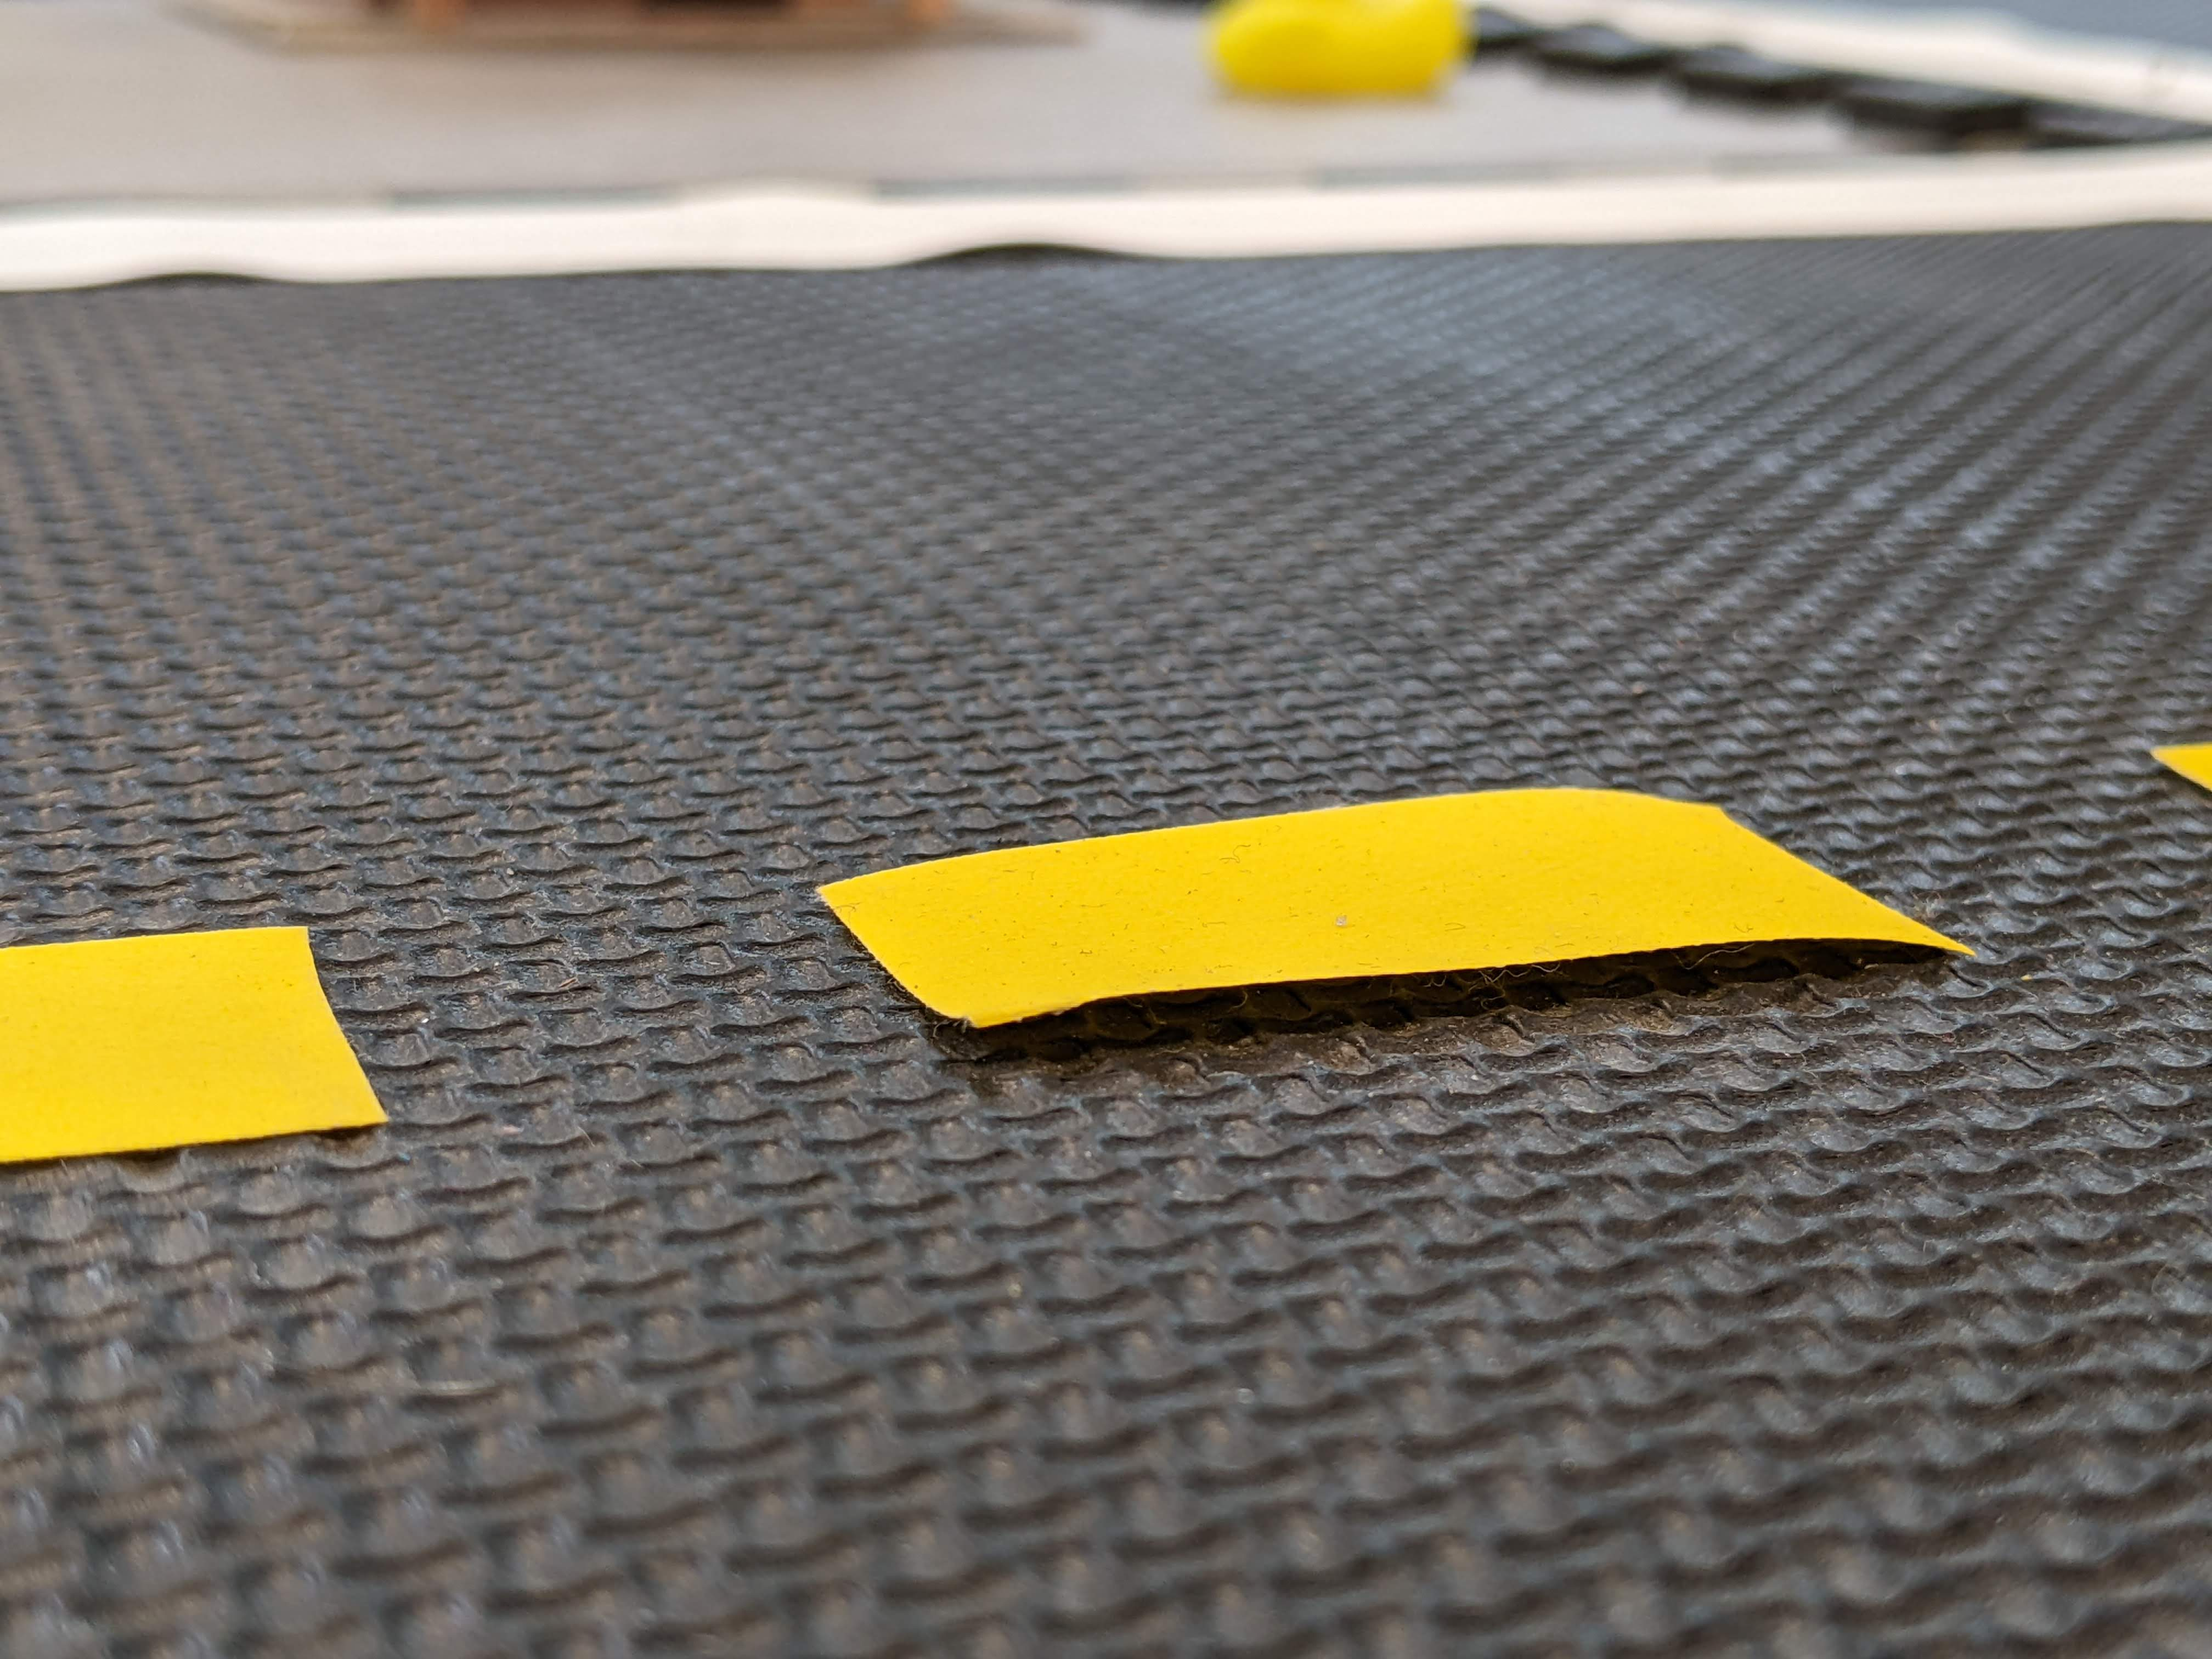
\includegraphics[width=0.4\textwidth]{floor-2.jpg}
    \\
    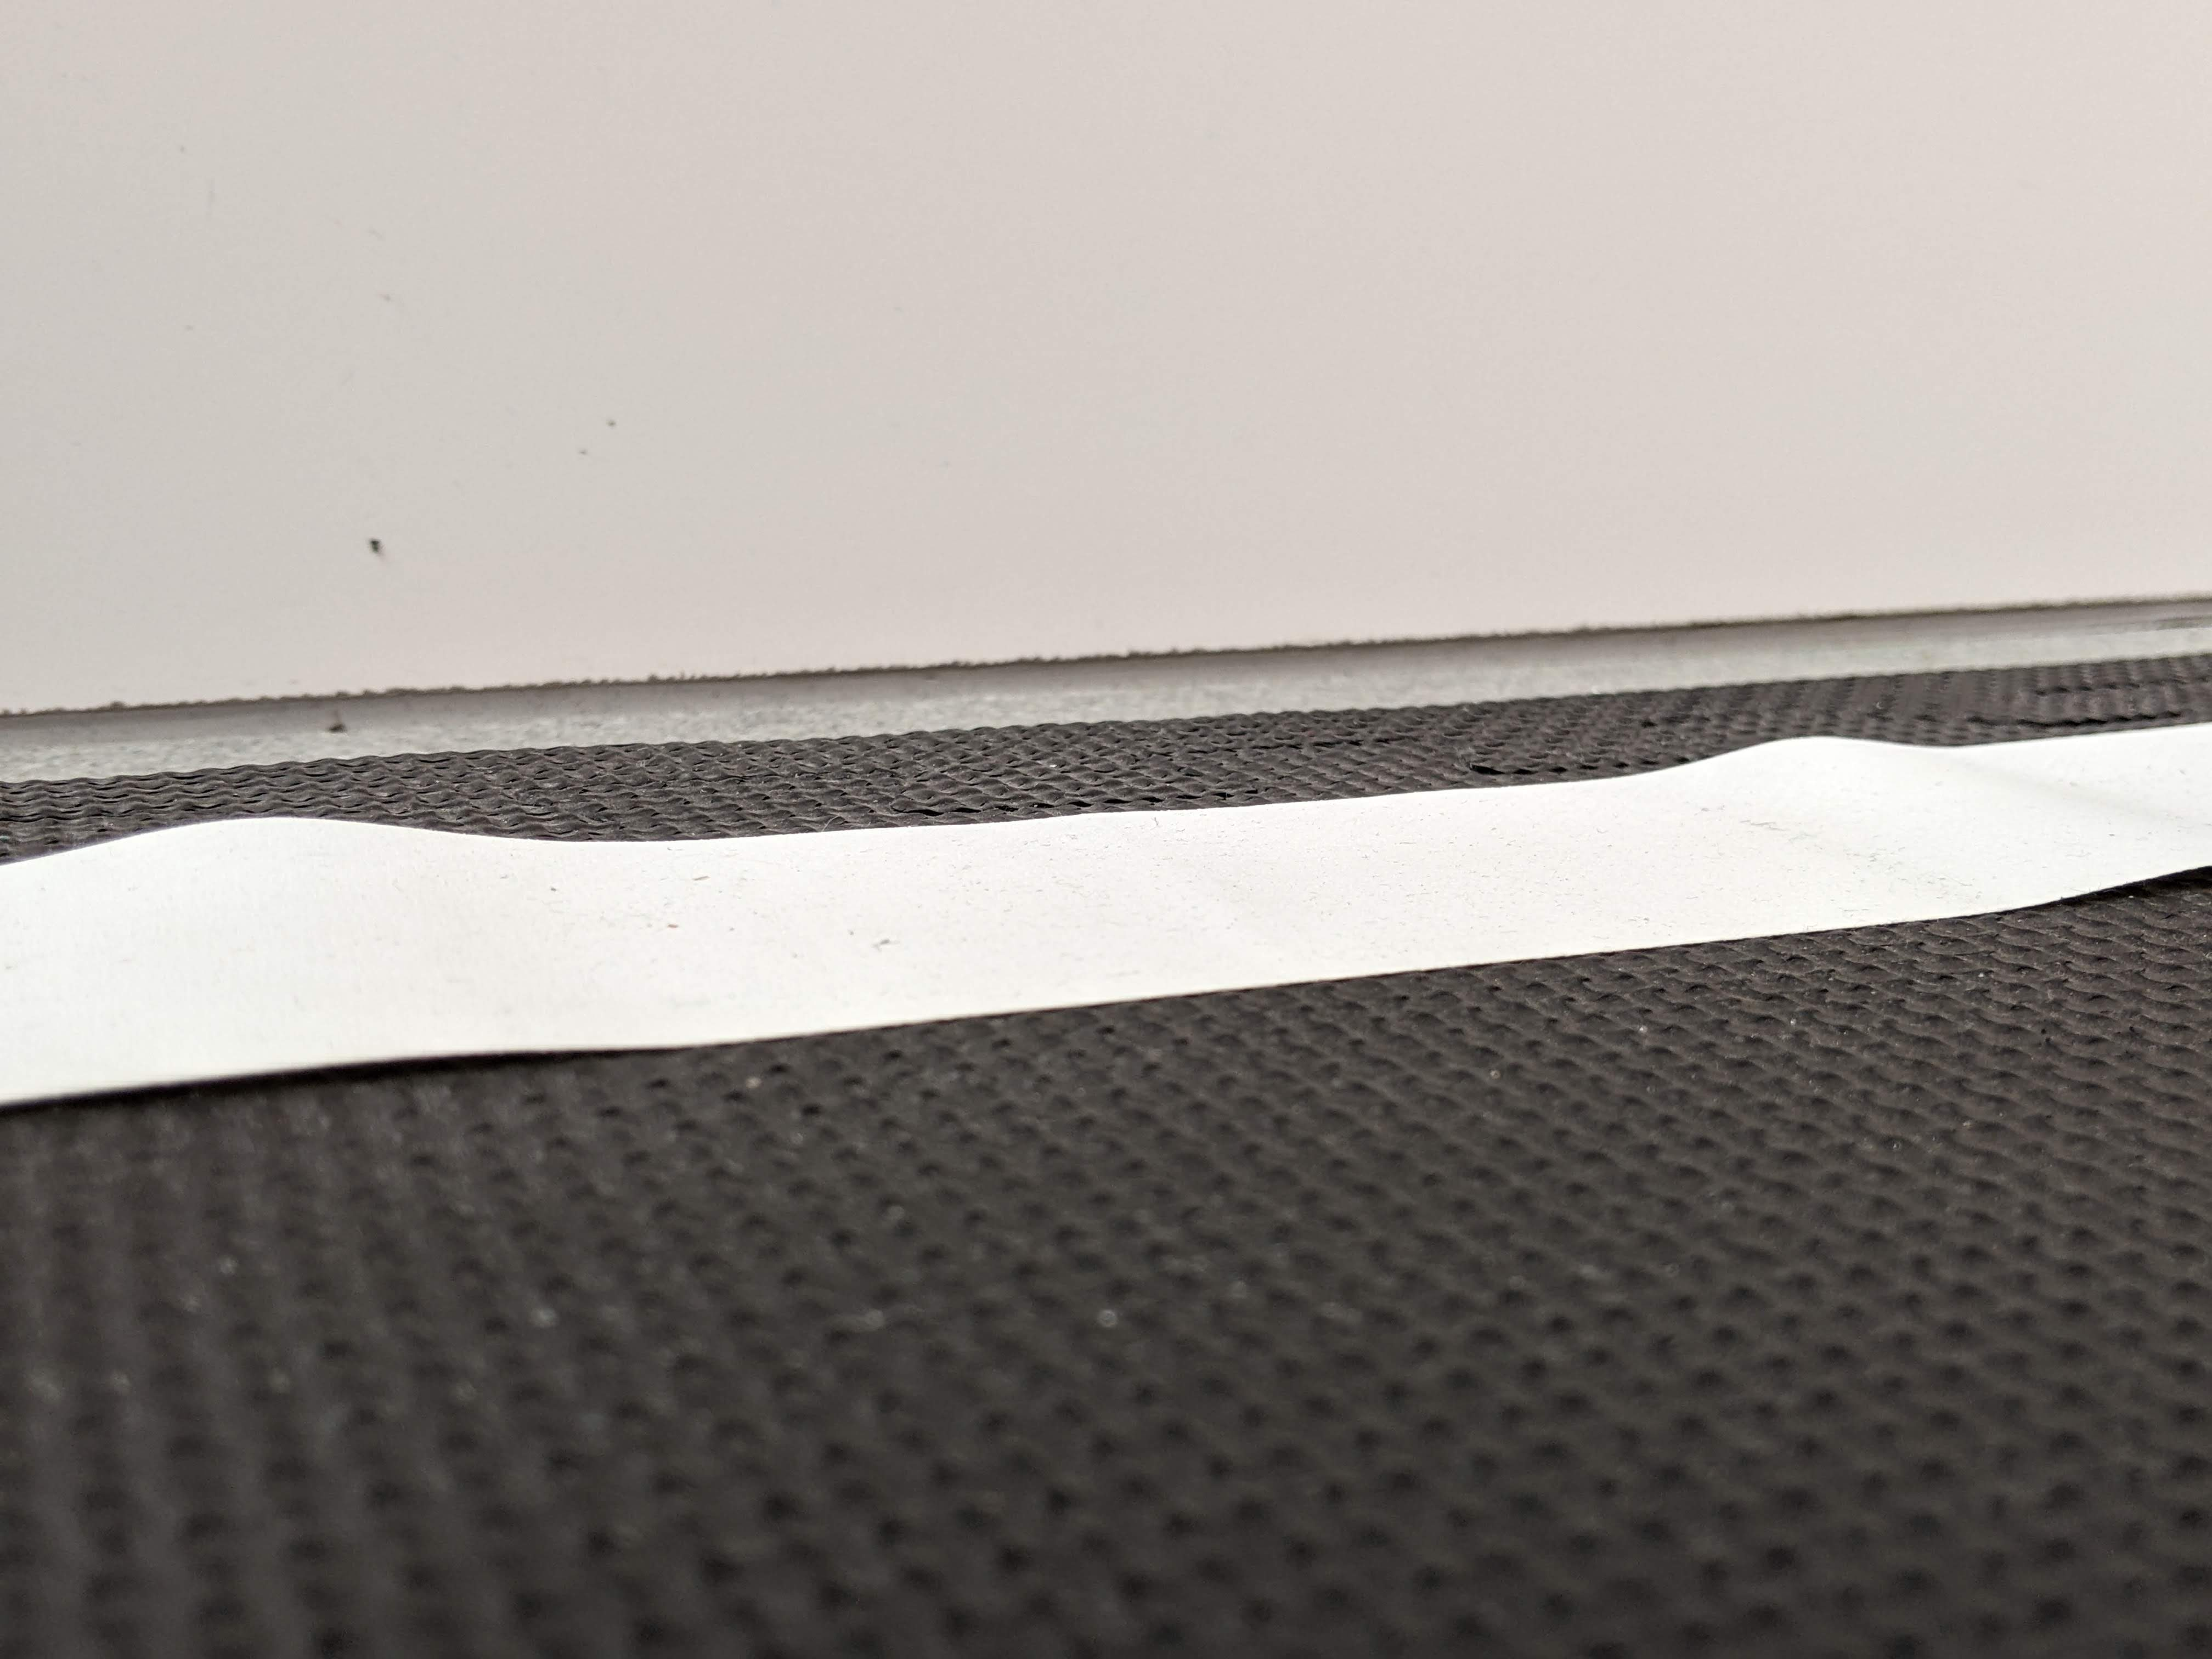
\includegraphics[width=0.4\textwidth]{floor-3.jpg}
    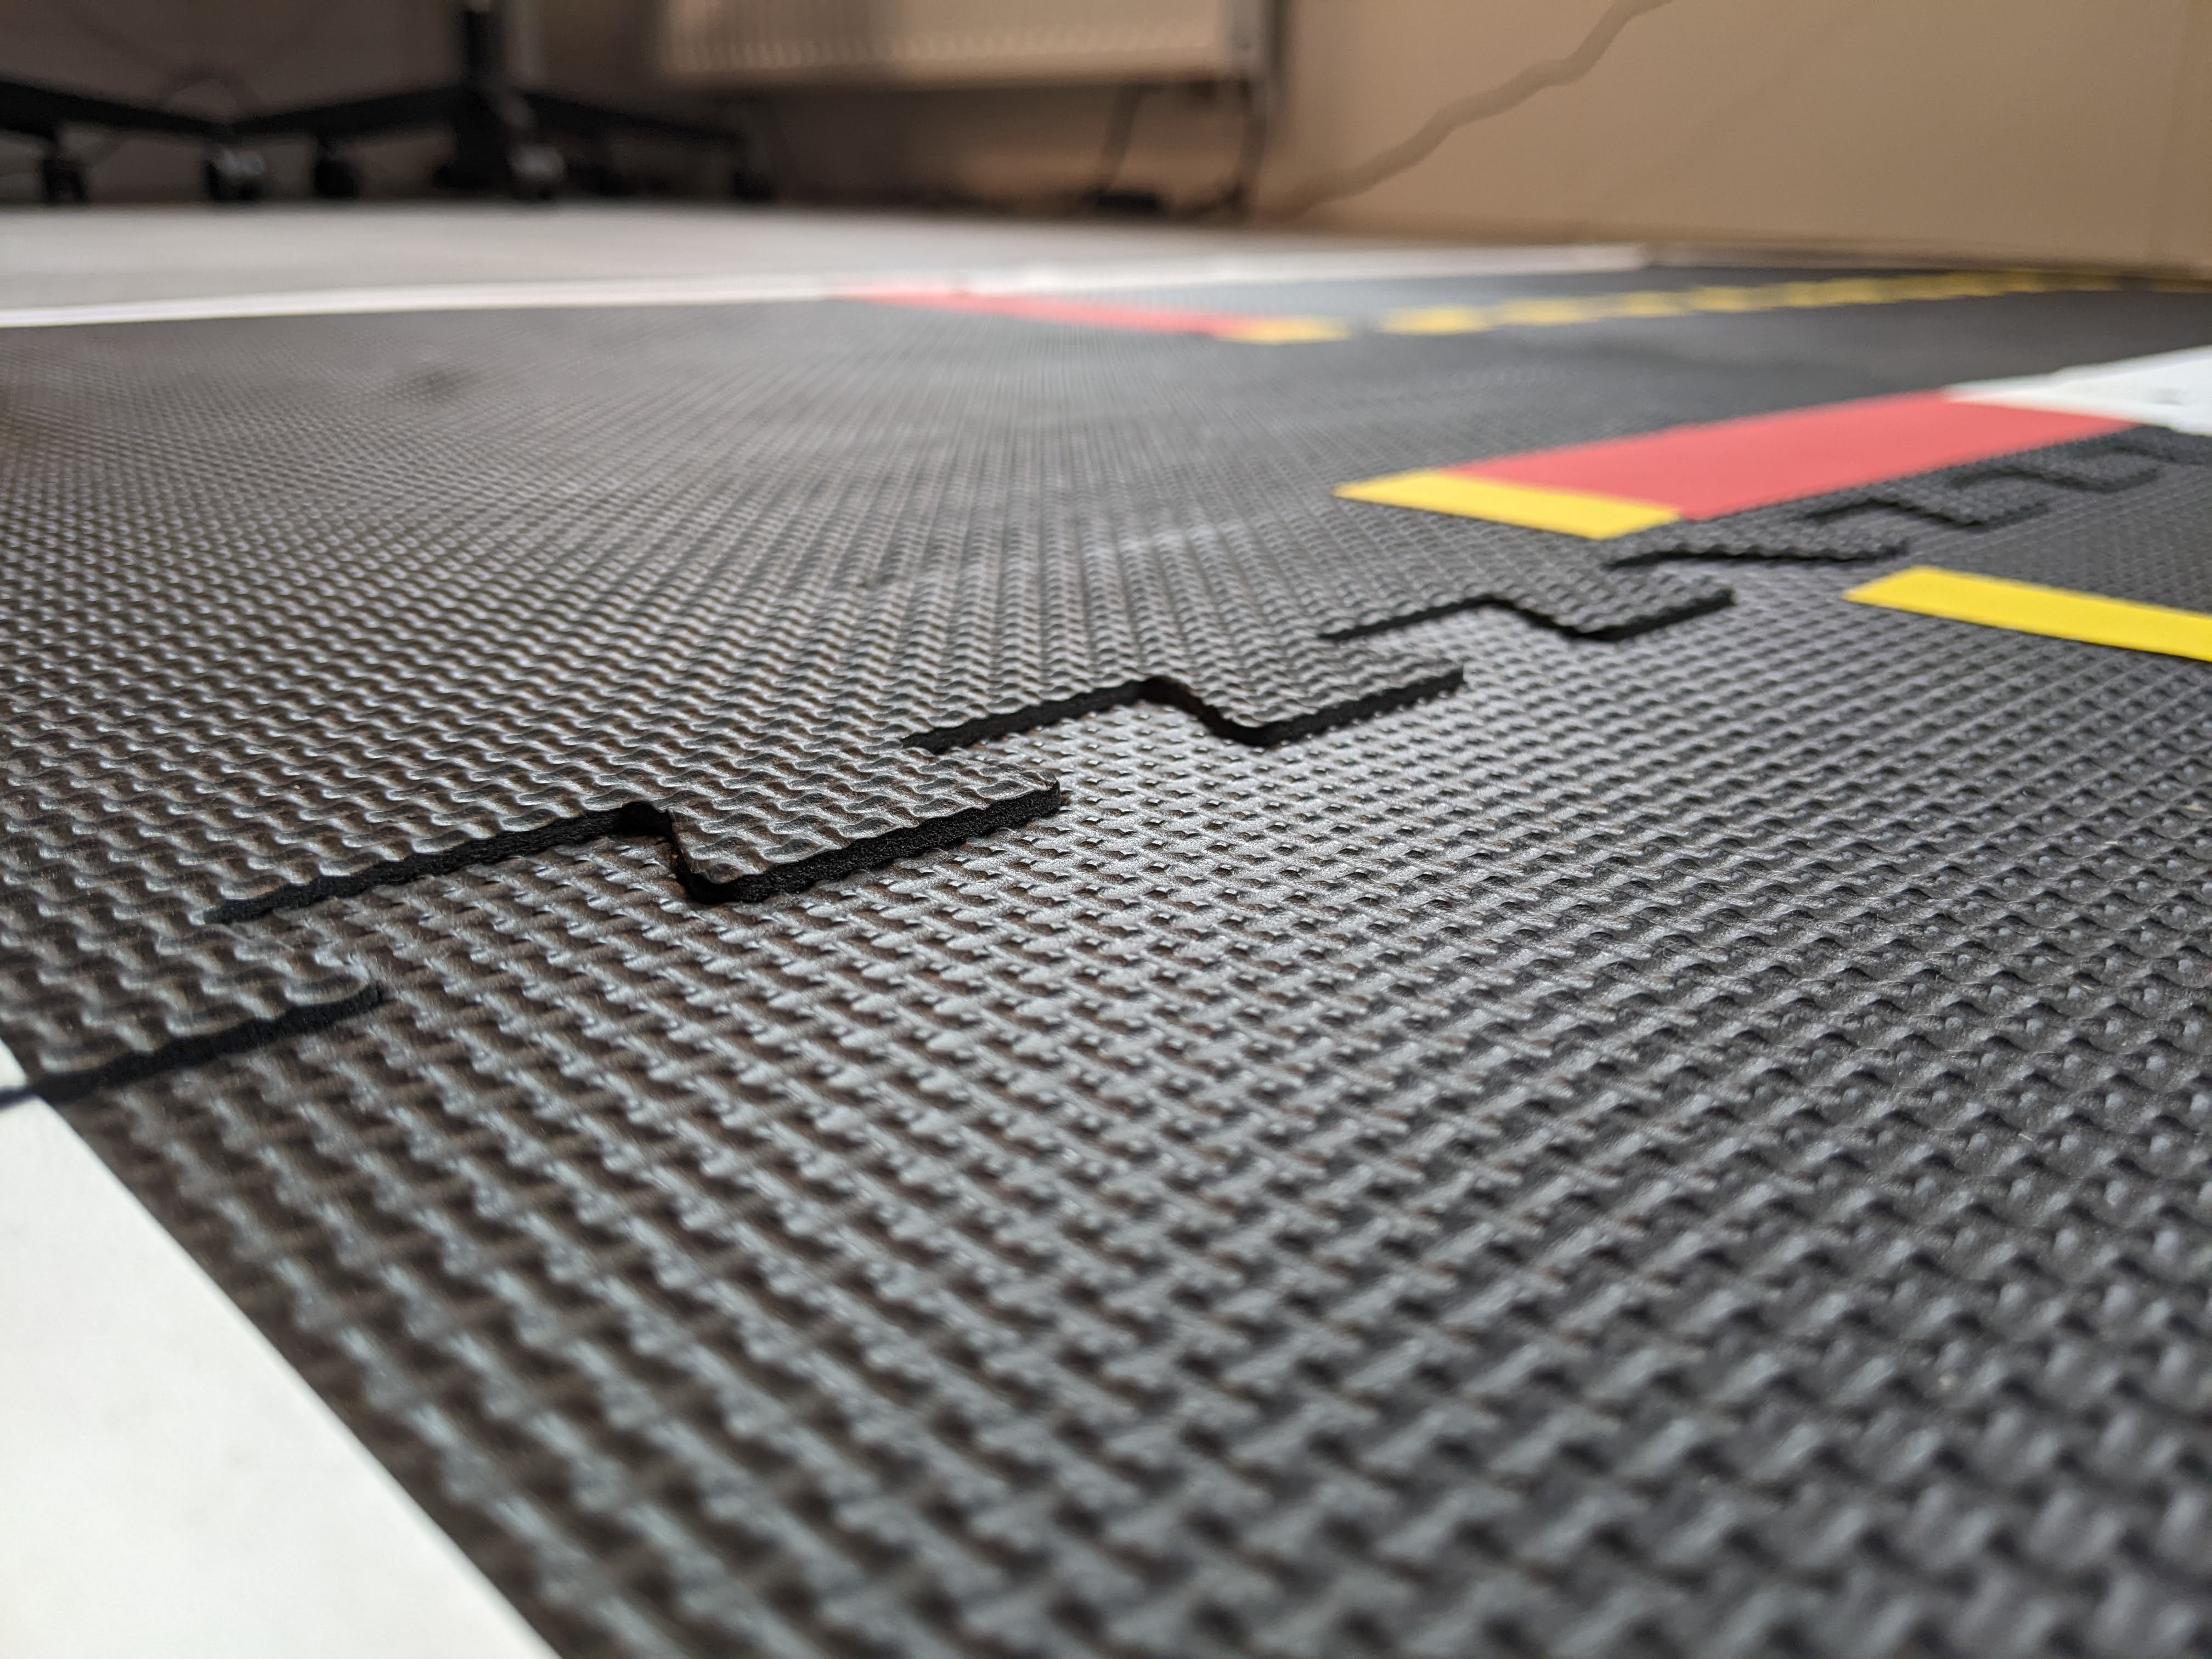
\includegraphics[width=0.4\textwidth]{floor-4.jpg}
    \caption{Makieta modelu projektu Duckietown.}
    \label{fig:smart-city-plan-1}
\end{figure}

Rozwiązaniem problemów z matą jest przede wszystkim zastosowanie innej taśmy niż ta którą sprzedaje fundacja Duckietown. Z pośród różnych taśm przetestowanych przez autorów najlepszymi właściwościami charakteryzowała się taśma firmy WELSTIK. Dodatkowo, przed przyklejeniem taśmy do panelu warto go wyczyścić np. izopropanolem lub innym płynem który w swoim składzie zawiera alkohol tak aby odtłuścić powierzchnię. Ostatnią operacją którą można wykonać jest podgrzanie przyklejonej taśmy wykorzystując np. suszarkę do włosów. 

\section{Software}\label{sec:software}
Niewątpliwie mocną stroną projektu Duckietown jest jego oprogramowanie do którego  wykorzystano najpopularniejszy obecnie framework do programowania robót -- Robot Operation System. 
Podział całego oprogramowania na poszczególne moduły i pakiety jest prawidłowy, zrozumiały i logiczny. 
Poszczególne elementy/moduły oprogramowania zrealizowane są z wykorzystaniem technologii konteneryzacji. Dzięki szerokiemu zastosowaniu konteneryzacji można łatwo, szybko i bezpiecznie tworzyć i testować własne oprogramowanie. Warto również zaznaczyć iż technologie wytwarzania oprogramowania wykorzystujące konteneryzację są obecnie bardzo popularne i często stosowane przy wytwarzaniu oprogramowania.  

Oprogramowanie projektu Duckietown zawiera również tzw. Duckie Town Shell. Jest to zestaw skryptów który ułatwia i automatyzuje różne czynności związane z bieżącą obsługą robotów Duckiebot np.: aktualizowanie oprogramowania, tworzenie obrazów dockera, uruchamianie kontenerów i wiele innych.

Stan w jakim znajduje się aktualnie robot Duckiebot może być sprawdzony za pomocą oprogramowania w przeglądarce internetowej. Każdy z robotów Duckiebot udostępnia taki interfejs w formie mikro-serwisu.

Roboty Duckiebot można programować w języku python lub C/C++ co jest konsekwencją wykorzystania frameworka ROS. Kod źródłowy oprogramowania robotów Duckiebot jest dostępny w postaci repozytorium na serwisie github\footnote{https://github.com/duckietown}.

W zasadzie jedyną wadą dostępnego obecnie programowania jest brak możliwości wykorzystania układu GPU w jaki wyposażony jest komputer NVIDIA Jetson Nano. Wynika to przede wszystkim z niekompatybilności wersji oprogramowania python, tensorflow. Możliwość wykorzystania sprzętowego układu GPU ma wpływ przede wszystkim na wykorzystnie sieci neuronowych do sterowania robotem Duckiebot.

\section{Dokumentacja}\label{sec:documentation}
Dokumentacja projektu Duckietown składa się dokumentów elektronicznych (w formacie html lub pdf)  w których w sposób łatwy i przystępny opisane są zagadnienia od montażu robota Duckiebot (krok po kroku), prawidłowego wykonania makiety, po zagadnienia związane z programowaniem robotów.
W dokumentacji można znaleźć wyczerpujące opisy architektury oprogramowania projektu Duckietown, bardzo dużo przykładów a także zaleceń postępowania w razie problemów. Dokumentacja projektu Duckietown jest również aktualizowana na bieżąco np. poprawiane są nieaktywne linki (po ich zgłoszeniu) a także jest ona uzupełniania o dodatkowe informacje.
Niestety dokumentacja projektu Duckiebot nie jest jeszcze kompletna, wielu jej miejscach brak jest treści które na razie nie są uzupełnianie.
W skład dokumentacji projektu Duckbietown wchodzą również materiały dydaktyczne w postaci wykładów, filmów, ćwiczeń a także obszernego kursu na platformie e-lerningowej edX pod tytułem "Self-Driving Cars with Duckietown". Przygotowane są również ćwiczenia w postaci skryptów jupyter oraz szablony repozytoriów github-a do wykorzystania w trakcie zajęć.

\section{Wnioski}\label{sec:conclusion}
W podsumowaniu należy stwierdzić, że projekt Duckietown pomimo swoich licznych wad jest projektem wartościowym. Niewątpliwie największą zaletą projektu Duckietown jest to, że stanowi on kompletny ekosystem w skład którego wchodzi: dokumentacja, oprogramowanie, sprzęt oraz środowisko symulacyjne umożliwiające efektywnie i nowoczesne nauczanie oraz prowadzenie zaawansowanych badań naukowych z zakresu robotów autonomicznych. 

Liczne wady dostrzeżone i opisane w artykule można w łatwy sposób skorygować we własnym zakresie. Należy również podkreślić, iż zarządzający projektem Duckietown po zgłoszeniu im problemów i zasugerowania rozwiązania na bieżąco aktualizują dokumentacje projektu o proponowane rozwiązania. 

W ocenie autorów najpilniejszymi rzeczami które powinny zostać poprawione to: konstrukcja mechaniczna nadwozia (lepsze materiały, inny sposób łączenie i mocowania różnych elementów), wymiana silników na inny model, aktualizacja oprogramowania tak aby możliwe było wykorzystanie sprzętowego układu GPU. Z czasem również koniecznością stanie się zastąpienie ROS jego nowszą wersją ROS2.


\bibliographystyle{plain}
\bibliography{references}

\end{document}
